\documentclass[12pt,a4paper]{report}
\setlength{\headheight}{21pt}

% ================== PACKAGE IMPORTS ==================
\usepackage{graphicx}
\usepackage{tabularx,adjustbox}
\usepackage{longtable,xtab}
\usepackage{tablefootnote,threeparttable}
\usepackage{multirow}
\usepackage{booktabs}
\usepackage{mathtools,amsmath,amssymb,amsfonts}
\usepackage{float}
\usepackage{xcolor}
\usepackage{siunitx}
\usepackage{csquotes}
\usepackage[acronym]{glossaries}
\usepackage[labelsep=period]{caption}
\usepackage{subcaption}
\usepackage{enumerate}
\usepackage{algorithm}
\usepackage{algpseudocode}
\usepackage{array,alphalph}
\usepackage{truncate}
\usepackage{fancyhdr,setspace}
\usepackage[sort,numbers]{natbib}
\usepackage{hyperref}
\usepackage{epstopdf}
\usepackage{pdfpages}
\usepackage{chngcntr}
\usepackage[english]{babel}
\usepackage{blindtext}
\usepackage{times}
\usepackage[toc,page,header]{appendix}
\usepackage{pifont}
\usepackage{titlesec}
\usepackage{geometry}
\usepackage{verbatim}
\usepackage{tikz}
\usepackage{listings}
\usepackage{microtype}
\usepackage[titles]{tocloft}

% Suppress overfull/underfull warnings
\hbadness=10000
\vbadness=10000
\hfuzz=2pt
\vfuzz=2pt
\emergencystretch=3em

\usetikzlibrary{positioning, shapes.geometric, shapes.symbols, arrows.meta, shadows, calc, fit, backgrounds, decorations.pathreplacing}

% ================== COLOR DEFINITIONS ==================
\definecolor{codegray}{gray}{0.95}
\definecolor{commentgreen}{rgb}{0,0.6,0}
\definecolor{keywordblue}{rgb}{0,0,1}
\definecolor{darkgray}{gray}{0.3}
\definecolor{auburn}{rgb}{0.43, 0.21, 0.1}
\definecolor{vividauburn}{rgb}{0.58, 0.15, 0.14}
\definecolor{bole}{rgb}{0.47, 0.27, 0.23}
\definecolor{midnightblue}{rgb}{0.1, 0.1, 0.44}
\definecolor{internationalkleinblue}{rgb}{0.0, 0.18, 0.65}
\definecolor{pipelineblue}{rgb}{0.18, 0.36, 0.58}
\definecolor{pipelinegreen}{rgb}{0.20, 0.55, 0.30}
\definecolor{pipelineamber}{rgb}{0.78, 0.50, 0.10}
\definecolor{pipelinered}{rgb}{0.65, 0.14, 0.14}
\definecolor{boxfill}{rgb}{0.93, 0.96, 1.0}

% ================== CODE LISTING STYLE ==================
\lstdefinestyle{mystyle}{
    backgroundcolor=\color{codegray},
    commentstyle=\color{commentgreen},
    keywordstyle=\color{keywordblue},
    numberstyle=\tiny\color{darkgray},
    stringstyle=\color{purple},
    basicstyle=\ttfamily\footnotesize,
    breaklines=true,
    numbers=left,
    numbersep=5pt,
    frame=single,
    tabsize=2
}
\lstset{style=mystyle}

% ================== PAGE STYLE ==================
\pagestyle{fancy}
\fancyhf{}
\fancyhead[R]{\fontsize{8}{8}\selectfont\itshape\nouppercase{\textcolor{internationalkleinblue}{\leftmark}}}
\fancyfoot[L]{\fontsize{8}{8}\selectfont\itshape\textcolor{internationalkleinblue}{PDEU}}
\fancyfoot[C]{\fontsize{6}{6}\selectfont\itshape\textcolor{internationalkleinblue}{V3 Positional Trading System -- Walk-Forward Validation \& Live Deployment}}
\fancyfoot[R]{\fontsize{8}{8}\selectfont\thepage}

\renewcommand{\headrulewidth}{2pt}
\renewcommand{\footrulewidth}{2pt}
\renewcommand{\headrule}{\hbox to\headwidth{\color{auburn}\leaders\hrule height \headrulewidth\hfill}}
\renewcommand{\footrule}{\hbox to\headwidth{\color{auburn}\leaders\hrule height \footrulewidth\hfill}}

\makeatletter
\let\ps@plain\ps@fancy
\makeatother

% ================== PAGE GEOMETRY (binding margins per guidelines) ==================
\geometry{
    a4paper,
    left=1.5in,
    right=1.0in,
    top=1.0in,
    bottom=1.0in,
    headheight=21pt
}

% ================== TITLE FORMATTING ==================
% Chapter Title: 20pt Bold  |  Headings: 14.4pt Bold  |  Subheadings: 12pt Bold
\titleformat{\chapter}[display]
    {\fontsize{20pt}{24pt}\selectfont\bfseries\color{auburn}}
    {\chaptertitlename\ \thechapter}{10pt}
    {\fontsize{20pt}{24pt}\selectfont\bfseries}
\titlespacing*{\chapter}{0pt}{-20pt}{20pt}

\titleformat{\section}
    {\fontsize{14.4pt}{17pt}\selectfont\bfseries\color{vividauburn}}
    {\thesection}{12pt}{}

\titleformat{\subsection}
    {\fontsize{12pt}{14pt}\selectfont\bfseries\color{bole}}
    {\thesubsection}{10pt}{}

% ================== SPACING: 1.5 line spacing, 12pt body font ==================
\onehalfspacing

% ================== HYPERREF SETTINGS ==================
\hypersetup{
    colorlinks=true,
    linkcolor=black,
    citecolor=black,
    urlcolor=black
}

% ================== TOLERANCE SETTINGS ==================
\hbadness=10000
\vbadness=10000
\hfuzz=5pt
\vfuzz=5pt
\emergencystretch=5em
\tolerance=9999
\pretolerance=8000
\raggedbottom

% ================== GRAPHICS PATH ==================
\graphicspath{{images/}{images/plots/}}

% ================== DOCUMENT START ==================
\begin{document}

% ========== FRONT MATTER ==========
% ================== FRONT MATTER ==================
    \pagestyle{plain}\clearpage
    \thispagestyle{empty}
    \begin{titlepage}
        \centering
        \vspace*{0.1cm}
    {\fontsize{17pt}{20pt}\selectfont \bfseries A Positional Trading System for the National Stock Exchange of India: \\ Walk-Forward Ensemble Learning, Calibrated Probabilities, and Live API Deployment}

        \vspace{0.5cm}
        {\large A Master's Thesis Report}
        \vspace{0.5cm}

        {\large Master of Technology in Artificial Intelligence}\\

        {\large by}\\

        {\Large\bfseries Vishwam K. Shah}

        {\large 24MAI022}\\
        \vspace{0.7cm}
       {\large Under the guidance of}\\
{\large \textbf{Dr. Jigarkumar Shah}}\\
{\large Department of Information and Communication Technology}\\

        \vspace{0.3cm}
        \vfill
        {\centering 
\includegraphics[width=0.21\textwidth]{pdeulogo.png}}\\
        {\large School of Technology}\\
        {\large Pandit Deendayal Energy University}\\
        {\large Gandhinagar -- 382426. Gujarat - India}\\
        {\large May, 2026}
    \end{titlepage}

    % Roman numbering for front matter
    \pagenumbering{roman}
    \clearpage
    \begin{center}
    \textbf{\large Approval Sheet}
    \end{center}

    This Project Report entitled \textbf{\enquote{A Positional Trading System for the National Stock Exchange of India: Walk-Forward Ensemble Learning, Calibrated Probabilities, and Live API Deployment}} by \textbf{Vishwam Shah} is recommended for the degree of \textbf{M.Tech} in \textbf{Artificial Intelligence}.
    \vspace{0.8cm}

    \hspace{9cm}Examiners
    \begin{flushright}
    \vspace{0.5cm}
     \vspace{0.5cm}
        \makebox[1.8in]{\hrulefill}\\
        Panel Member 1,\\
         \vspace{0.5cm}
         \makebox[1.8in]{\hrulefill}\\
        Panel Member 2,\\
         \vspace{0.5cm}
          \makebox[1.8in]{\hrulefill}\\
        Panel Member 3,\\
        \vspace{0.5cm}
         \makebox[1.8in]{\hrulefill}\\
        Dr. Jigarkumar Shah,\\
         \makebox[1.8in]{\hrulefill}\\
        Dr. Paawan Sharma,\\
         HOD, ICT \\
    \end{flushright}
    \vspace{0.5cm}
    \vfill

    \newpage
    \begin{center}
	    \textbf{\large Student Declaration}
    \end{center}

    I, \textcolor{internationalkleinblue}{\textbf{Vishwam Shah}}, hereby declare that this written submission represents my ideas in my own words, and where others' ideas or words have been included, I have adequately cited and referenced the original sources. I also declare that I have adhered to all principles of academic honesty and integrity and have not misrepresented or fabricated, or falsified any idea/data/fact/source in my submission. I further declare that all software artefacts, model checkpoints, probability calibration outputs, walk-forward result tables, paper-trading session logs, and backtest equity curves cited in this thesis were generated by code that is part of the accompanying source repository, and that the figures reproduce these artefacts without manual alteration. I understand that any violation of the above will be cause for disciplinary action by the Pandit Deendayal Energy University.
    \vspace{0.8cm}
    \vspace{0.8cm}
    \begin{flushright}
        \makebox[1.8in]{\hrulefill}\\
        Vishwam Shah\\
        Roll No: 24MAI022\\
    \end{flushright}
    \vfill
    \begin{flushleft}
	    Date: \makebox[1.8in]{\hrulefill}
    \end{flushleft}

    % Acknowledgment section
    \section*{\textbf{Acknowledgment}}
    I would like to express my sincere gratitude to my supervisor \textbf{Dr.\ Jigarkumar Shah}, Department of Information and Communication Technology, for his consistent guidance, patience, and constructive feedback throughout the V3 redesign of this system --- particularly during the move from a single-model prototype to a ten-model parallel ensemble, the introduction of expanding-window walk-forward validation, and the build-out of the live trading layer. His insistence on leakage audits, calibrated probabilities, and brokerage-aware promotion gates shaped the engineering discipline of this work. I thank the Head of Department \textbf{Dr.\ Paawan Sharma} for departmental support, and the faculty of the M.Tech (Artificial Intelligence) programme at PDEU for an academic environment where systematic experimentation was encouraged over headline metrics. I am grateful to my parents for their continuous moral and material support during the long compute runs and the inevitable debugging cycles of a 100-stock production pipeline.

    \begin{flushright}
    \textbf{Vishwam Shah}\\
    \end{flushright}

    % Abstract
    \chapter*{Abstract}
    \addcontentsline{toc}{chapter}{Abstract}
    \pagestyle{fancy}
    This thesis presents \textbf{V3}, a production-grade positional trading system for the Indian equity market, evaluated on \textbf{99 of 100 large-capitalisation NSE stocks} (one constituent skipped automatically due to insufficient post-feature history) spanning the Nifty-50 and Nifty Next-50 universes. The system trains a heterogeneous ensemble of \textbf{ten classifiers} per stock --- LightGBM, XGBoost, LSTM, BiLSTM, GRU, CNN-LSTM, CNN-GRU, TCN-GRU, TCN-Transformer and N-BEATS --- under a \textbf{zero-leakage expanding-window walk-forward protocol} with \textbf{six chronological folds} per symbol, fits a logistic-regression meta-learner on out-of-fold tree probabilities, and applies \textbf{single-parameter temperature scaling} on the validation slice to produce calibrated next-day-direction probabilities.

    On the latest full run (run id \texttt{20260505\_153704}, \(99\) symbols, \(62{,}212\) out-of-sample predictions across all folds), the system attains a \textbf{mean out-of-sample accuracy of 51.45\%} on the raw $0.5$ decision rule and, restricted to high-confidence signals (\textit{calibrated probability} $>0.58$ and predicted move $>0.4\%$), a \textbf{bootstrap accuracy of 60.33\%} with a 95\% confidence interval of $[57.99\%,\ 62.81\%]$ over $1{,}495$ signal-days. The bootstrap interval excludes 50\%, establishing statistical significance versus a random baseline.

    Translated into a portfolio backtest from 30 November 2023 to 27 April 2026 (covering roughly two-and-a-half years of out-of-sample trading days), the long-only, top-15 cross-sectional ranked strategy produces a \textbf{total return of 225.5\%} versus a Nifty-50 buy-and-hold return of \textbf{18.7\%} over the same window, with a \textbf{Sharpe ratio of 1.656} and a \textbf{maximum drawdown of 21.5\%}. Diebold--Mariano tests against three na\"ive baselines (always-up, five-day momentum, AR(1)) show that the model is significantly better than the momentum and AR(1) baselines at the pooled level ($p < 0.001$). Regime-conditional diagnostics show the system is profitable across bull (Sharpe 2.65), sideways (Sharpe 1.93) and bear (Sharpe 2.26) regimes, with bear-market performance being the strongest contributor to absolute return.

    Methodologically, the contribution is fourfold. First, a \textbf{leakage-audited} feature pipeline that combines \(\sim\)200 OHLCV-derived features with global cues (S\&P 500, Nasdaq, US VIX, DXY, crude, Nikkei) merged using a strict prior-day \texttt{merge\_asof} and an NSE-specific calendar (F\&O expiry, RBI MPC dates, Union Budget dates, result-season indicator). Second, a \textbf{sector-aware feature force-include policy} that pins USD/INR and Nasdaq features for IT stocks and RBI/Crude/DXY features for banking. Third, \textbf{calibrated ensembling} that wraps a validation-fitted temperature scalar around a tree+DL+meta probability so that 58\% confidence corresponds to an empirically reliable probability rather than an arbitrary score. Fourth, a complete \textbf{live deployment layer}: an Angel One SmartAPI client, a paper-trading runner with realistic Indian brokerage modelling (STT, SEBI, GST, exchange charges, slippage), an automated \textbf{promotion gate} that blocks live capital until paper-trading meets pre-registered KPIs ($\geq 40$ closed trades, $\geq 20$ paper days, rolling Sharpe $\geq 1.0$, rolling drawdown $\leq 10\%$, slippage $\leq 25$bps, fill rate $\geq 90\%$, Brier-score drift $\leq 0.05$), and a Vite/React/FastAPI dashboard for human-in-the-loop monitoring. As of the most recent evaluation, the promotion gate evaluates to a \texttt{no-go} decision, correctly preventing real-money trading until paper-trading evidence accumulates.

    The system is reproducible: every run writes an immutable configuration record (pinning the random seed, train ratios, gating thresholds and feature flags), preserves per-window model checkpoints, and emits structured output files for the per-symbol summary, all fold details, the backtest portfolio, diagnostics, and next-day predictions. The complete source code, the 99-symbol per-run results, and the \(\sim\)$13{,}000$ paper-trade ledger entries are part of the accompanying repository.
    \clearpage

    % Table of contents
    \addcontentsline{toc}{chapter}{Contents}
    \tableofcontents
    \addcontentsline{toc}{chapter}{List of Figures}
    \listoffigures
    \addcontentsline{toc}{chapter}{List of Tables}
    \listoftables

    % Start main content with Arabic numbering
    \cleardoublepage\pagenumbering{arabic}
    \pagestyle{fancy}


% ========== TABLE OF CONTENTS / LOF / LOT ==========
\pagestyle{fancy}
\addcontentsline{toc}{chapter}{Contents}
\tableofcontents

\clearpage
\pagestyle{fancy}
\addcontentsline{toc}{chapter}{List of Figures}
\listoffigures

\clearpage
\pagestyle{fancy}
\addcontentsline{toc}{chapter}{List of Tables}
\listoftables

\cleardoublepage
\pagenumbering{arabic}
\pagestyle{fancy}

% ========== CHAPTER 1: INTRODUCTION ==========
\chapter{Introduction} \label{chapter1}

\section{Problem Statement}

The forecasting of next-day directional movements in equity prices is a long-standing problem at the intersection of statistical learning and market microstructure. From a deployment perspective the practical question is not whether a forecaster can attain an impressive in-sample $R^2$, but whether a probability output, when filtered through a confidence threshold and routed through a real Indian-market broker (with brokerage, exchange charges, Securities Transaction Tax, GST, SEBI levy, stamp duty, and realistic slippage), \emph{net} of all these frictions and on stochastically unseen out-of-sample days, produces a positive risk-adjusted return curve. This thesis develops, audits, and deploys such a system on the \textbf{Nifty-100 universe of the National Stock Exchange (NSE) of India}.

The work was motivated by three observations from an earlier prototype of the same system (subsequently archived as the V2 prototype) and from the published Indian-market literature.

\begin{enumerate}
    \item \textbf{Headline accuracies in the literature are inflated by leakage and test-set construction.} Reported direction accuracies in the 60--70\% range for Indian stocks frequently rely on random train--test splits, on scalers fitted across the full panel, on labels created \emph{before} the split (which then leak into the test set through any forward-looking rolling statistic), or on a single contiguous test slice in which the model happens to ride a benign regime. The first version of this work reported 68.28\% direction accuracy on 106 stocks using a 60/20/20 chronological split; the same code, replayed under expanding-window walk-forward validation with $K = 6$ folds per symbol and the scaler refit per fold, settles to a mean accuracy in the low-50\%s. Both numbers are correct; the difference is the protocol.
    \item \textbf{Tree models dominate tabular OHLCV; deep sequence models contribute only when used jointly.} On individual stocks, LightGBM and XGBoost consistently outperform LSTM/GRU/BiLSTM. However, deep models contribute non-trivial diversification when stacked with a logistic-regression meta-learner; we therefore train both families and let a learnt meta-learner blend them rather than discarding the deep stack on the basis of marginal solo accuracy.
    \item \textbf{The economically interesting signal is not the raw accuracy --- it is the conditional accuracy at high calibrated confidence.} A 51.5\% all-days accuracy that becomes 60.3\% on the 1{,}495 signal-days at which calibrated probability exceeds $0.58$ \emph{and} the predicted absolute move exceeds 40bps (the round-trip transaction cost) is operationally very different from a 51.5\% all-days accuracy with no gating. The gating decision is the deployable artefact.
\end{enumerate}

\section{Goals and Contributions}

The V3 system has four design goals, each of which corresponds to a contribution of this thesis.

\subsection*{G1. Leakage-audited features}
\textbf{Goal.} Build a feature engineering layer such that any feature used at decision time $t$ depends \emph{only} on data observable strictly before the NSE open of day $t$. \textbf{Contribution.} A documented audit of every feature family: target is constructed with a single \texttt{shift(-1)} \emph{after} all features are computed; the \texttt{RobustScaler} and the PCA fit are computed on the training window only; the global cues (S\&P 500, Nasdaq, US VIX, DXY, Crude, Nikkei) are shifted by one calendar day and merged into the Indian time series with \texttt{merge\_asof(direction=\textquotesingle backward\textquotesingle, strict prior)}, so that the Indian decision on date $t$ sees only the US close of $t-1$.

\subsection*{G2. Heterogeneous ensemble with calibrated probability}
\textbf{Goal.} Train an ensemble whose member errors are decorrelated, and produce a probability rather than a margin. \textbf{Contribution.} Five models per symbol, namely two gradient boosters (LightGBM, XGBoost) and three deep sequence models (BiLSTM, TCN-Transformer, N-BEATS), combined by a logistic-regression meta-learner on out-of-fold tree probabilities. A single-parameter \textbf{temperature scaling}~\cite{guo2017calibration} is fitted on the validation slice and applied at inference, producing a probability whose reliability has been verified by a per-symbol calibration curve.

\subsection*{G3. Expanding-window walk-forward validation}
\textbf{Goal.} Quantify performance under the protocol that most closely matches deployment. \textbf{Contribution.} Six chronological folds per symbol with train ratio expanding from $0.70$ to $0.95$ in steps of $0.05$, with the scaler and PCA refit per fold. Aggregation across the $100 \times 6$ window grid yields $67{,}830$ out-of-sample predictions covering roughly two-and-a-half years of unseen trading days.

\subsection*{G4. Live deployment with brokerage-aware promotion gate}
\textbf{Goal.} Make it impossible for real money to flow into the strategy unless paper-trading evidence meets pre-registered KPIs. \textbf{Contribution.} A complete live layer: an Angel One SmartAPI client; a paper-trader with explicit Indian-market cost modelling (STT, exchange charges, GST, SEBI, stamp duty, slippage); an automated \texttt{PromotionGate} (\(\geq 40\) closed trades, \(\geq 20\) paper days, rolling Sharpe \(\geq 1.0\), rolling drawdown \(\leq 10\%\), fill rate \(\geq 90\%\), slippage \(\leq 25\)bps, Brier-score drift \(\leq 0.05\)); and a Vite/React/FastAPI dashboard for human-in-the-loop oversight. The gate currently evaluates to \texttt{no-go}, correctly blocking live capital while paper evidence accrues.

\section{Scope and Universe}

The system is evaluated on the Nifty-100 large-capitalisation universe. After a minimum-history filter, \textbf{all 100 symbols} from the Nifty-50 and Nifty Next-50 universes are admitted on the latest full run. The data range is from \textbf{1 January 2018} to the run date; on the canonical run analysed in this thesis, the latest training window ends in late April 2026.

Coverage spans 14 sectors (banking, IT, automobiles, FMCG, pharma, energy, metals, telecom, capital goods, cement, consumer durables, real estate, conglomerate / infra, defense), reflecting the cross-section of the Indian large-cap market. The sectoral allocation and the live broker layer are India-specific, but the modelling layer is portable: the same five-model ensemble and the same walk-forward protocol can be lifted onto any equity universe with daily OHLCV plus exogenous cues.

\section{Distinction from the V2 Prototype}

The reader is referred for context to the predecessor system (the V2 prototype thesis), which reported a 68.28\% direction accuracy on 106 stocks using a 60/20/20 chronological split with four models (XGBoost, LSTM, GRU, Ridge-stacker). The differences are summarised in Table~\ref{tab:v2_vs_v3}; the operational gap is that the V2 number is the \emph{single-fold} accuracy under a benign regime, whereas the V3 numbers in this thesis are the \emph{six-fold expanding-window} accuracy aggregated over a multi-regime, $\sim$2.5-year out-of-sample period, on a larger model committee, with a leakage audit and live brokerage modelling that the V2 system did not implement.

\begin{table}[H]
\centering
\caption{V2 prototype versus V3 system}
\label{tab:v2_vs_v3}
\renewcommand{\arraystretch}{1.35}
\begin{adjustbox}{max width=\textwidth}
\begin{tabular}{l l l}
\toprule
\textbf{Dimension} & \textbf{V2 (archive)} & \textbf{V3 (this thesis)} \\
\midrule
Universe                  & 106 stocks, 11 sectors                                    & 100 NSE Nifty-100 (Nifty-50 + Next-50), 14 sectors \\
Validation protocol       & 60/20/20 single chronological split                        & Six-fold expanding-window walk-forward, train 0.70$\to$0.95 \\
Train/scale leakage audit & Not enforced (single scaler fit)                          & Scaler + PCA fit per fold, target by \texttt{shift(-1)} only \\
Model committee           & 4 (XGB, LSTM, GRU, Ridge-stack)                            & 5 (LGBM, XGB, BiLSTM, TCN-Transformer, N-BEATS) \\
Meta-learner              & Ridge regression                                          & Logistic regression on out-of-fold tree probs \\
Probability calibration   & None                                                      & Per-fold temperature scaling on val \\
Exogenous cues            & Optional, market-context disabled                          & Global cues + NSE calendar, force-included by sector \\
Gating                    & Single confidence threshold                               & MIN\_MOVE $\geq 0.4\%$ \emph{and} calibrated prob $\geq 0.58$ \\
Live layer                & Not present                                               & Angel One SmartAPI, paper-trader, automated promotion gate, dashboard \\
Reported headline         & 68.28\% direction acc (single split)                       & 51.25\% mean OOS acc (67{,}830 preds); 60.33\% on 1{,}495 high-confidence signals (bootstrap CI $[57.99, 62.81]$) \\
Portfolio backtest        & Not run end-to-end on the panel                            & Total return 225.5\%, Sharpe 1.656, max DD 21.5\% over $\sim$2.5 yrs \\
\bottomrule
\end{tabular}
\end{adjustbox}
\end{table}

\section{Organisation of the Thesis}

The remainder of this report is organised as follows. \textbf{Chapter~\ref{chapter2}} reviews the relevant literature on supervised forecasting of equity direction, focussing on Indian-market work, on lookahead-bias guidance from L\'opez de Prado~\cite{prado2018walkforward}, on the gradient-boosting versus deep-recurrent contrast, and on probability calibration. \textbf{Chapter~\ref{chapter3}} describes the V3 pipeline in detail: data acquisition, feature engineering (with the global-cues and NSE-calendar additions), the five-model committee, the walk-forward protocol, the meta-learner, and the temperature-scaling calibration. \textbf{Chapter~\ref{chapter4}} presents the results of the latest full run (\texttt{20260513\_164028}): aggregate accuracy on $67{,}830$ out-of-sample predictions, the high-confidence bootstrap interval on $1{,}495$ signal-days, the cross-sectional top-15 portfolio backtest (225.5\% total return), regime-conditional diagnostics, Diebold--Mariano significance tests, and per-symbol tables. \textbf{Chapter~\ref{chapter5}} documents the live trading layer: the broker client, the paper-trading runner, the cost model, the promotion gate, and the dashboard. \textbf{Chapter~\ref{chapter6}} discusses what the system does well, what it does poorly, and the immediate roadmap. The appendix lists the complete 100-symbol per-stock summary (Appendix A), the full configuration, the Angel One workflow, and a description of every CSV/JSON artefact produced per run.


% ========== CHAPTER 2: LITERATURE SURVEY ==========
\chapter{Literature Survey} \label{chapter2}

\section{Scope of the Survey}

This chapter reviews the literature that is load-bearing for the V3 design: (i) the directional forecasting problem and the random-walk null; (ii) supervised learning for tabular financial features (gradient boosting); (iii) deep sequence models for daily OHLCV; (iv) ensembling and meta-learning; (v) probability calibration; (vi) backtest hygiene and lookahead bias; (vii) macro / exogenous cues relevant for the NSE; (viii) Indian-market specific studies. Each subsection ends with a short note on the design implications for V3.

\section{The Directional Forecasting Problem and the EMH Null}

The semi-strong form of the Efficient Market Hypothesis~\cite{fama1970emh} implies that, conditional on public information, expected next-day excess returns are zero. Empirically, however, the literature shows that the joint hypothesis of zero predictability is rejected for short horizons under specific conditioning sets: weekly momentum~\cite{jegadeesh1993momentum}, post-earnings drift, market-microstructure inefficiencies, and macro-cue spillover from the US session into the Asian open. The V3 task is therefore not whether prices are predictable in general but whether \emph{a measurable subset of trading days carries enough conditional structure} for a learnt classifier to beat the round-trip cost.

\textbf{Implication for V3.} The gate is set so that the model is only allowed to trade on days where calibrated probability exceeds $0.58$ \emph{and} the predicted absolute move exceeds the round-trip cost ($\sim 0.4\%$ for NSE delivery). The reported headline number on all days (51.25\%) is consistent with weak-form efficiency; the headline number on signal days (60.33\%) is the figure that matters operationally.

\section{Gradient Boosting for Tabular Finance}

\textbf{XGBoost}~\cite{chen2016xgboost} introduced regularised tree boosting with second-order Taylor optimisation, sparsity-aware split-finding, and weighted quantile sketches. \textbf{LightGBM}~\cite{ke2017lightgbm} replaced level-wise growth with leaf-wise growth, gradient-based one-side sampling, and histogram-based feature bucketing, lowering wall-clock cost on wide tabular data without surrendering accuracy. On panel-style daily OHLCV with hand-engineered features, gradient boosting variants consistently outperform un-engineered deep nets~\cite{shwartz2022tabular,grinsztajn2022treesvsdl}. Both libraries handle missing values natively and tolerate heterogeneous feature scales without normalisation, which is convenient when ratios, percentages and raw indices coexist in the same matrix.

\textbf{Implication for V3.} V3 trains LightGBM and XGBoost on the post-PCA scaled matrix, with explicit $\ell_1$ and $\ell_2$ regularisation ($\alpha=0.3$, $\lambda=1.5$), a 1{,}000-tree budget, learning rate $0.01$, depth 5, and early stopping after 50 non-improving rounds. These two trees provide the meta-learner's feature space.

\section{Deep Sequence Models on Daily OHLCV}

The LSTM~\cite{hochreiter1997lstm} and the GRU~\cite{cho2014gru} were the first sequence architectures with controlled long-range gradient flow. Their direct application to financial time series~\cite{fischer2018lstm,sezer2020survey} produces respectable equity-curve numbers but mediocre out-of-sample direction accuracies once leakage is removed. Bidirectional variants are admissible here because every feature is lagged (no peek through Bi-direction). Convolutional preprocessing (CNN--LSTM, CNN--GRU) lifts local pattern extraction off the recurrent stack and is causal-padded to preclude future-step leakage. Temporal Convolutional Networks~\cite{bai2018tcn} replace the recurrence with dilated causal convolutions and have receptive field $1 + (k-1) \cdot 2 \sum d_i$, which for kernel size 3 and dilations $\{1, 2, 4, 8\}$ is $\sim 61$ time steps, comfortably wider than the 20-step sequence we feed in. N-BEATS~\cite{oreshkin2020nbeats} introduced residual backcast blocks for univariate forecasting; we adapt the generic configuration with a sigmoid classification head. Lim et al.'s Temporal Fusion Transformer~\cite{lim2021tft} influenced our \texttt{TCN-Transformer} block, which composes TCN local feature extraction with multi-head self-attention.

\textbf{Implication for V3.} Eight deep-learning models are trained per symbol per window with identical input shapes $(B \times 20 \times d)$ (batch size $B$, sequence length 20, feature dimension $d$), fed from the robust-scaled matrix. They consume the same input as the trees but contribute independently to the meta-learner, providing decorrelated error structure rather than competing for raw accuracy.

\section{Ensembling, Stacking, and the Meta-Learner}

\textbf{Stacked generalisation}~\cite{wolpert1992stacking} feeds out-of-fold predictions of base learners into a level-2 model that learns the optimal blend. The level-2 model should be simple to avoid further overfit; logistic regression is the canonical choice for binary stacking. The variance-reduction case for heterogeneous ensembles is made by Dietterich~\cite{dietterich2000ensemble}, who distinguishes bagging (same model, different data), boosting (sequential error-correction) and stacking (different model classes, learned blend). Heterogeneity is the only one of the three that gives V3 a structurally different error signal across families; bagging is implicit inside each booster, boosting is implicit inside each booster, and stacking is the V3 layer.

\textbf{Implication for V3.} V3 stacks the two tree probabilities (and optionally the deep-learning probabilities, when their validation accuracy clears a sanity floor) via logistic regression on out-of-fold tree predictions on the validation slice, producing a combined meta-probability at inference.

\section{Probability Calibration}

A classifier can rank the right way and still mis-state its probabilities. Modern deep networks in particular are systematically over-confident~\cite{guo2017calibration}. Two corrections dominate the literature: Platt scaling (a single logistic regression on the validation set's logits) and isotonic regression (a non-parametric monotonic fit). \textbf{Temperature scaling}~\cite{guo2017calibration} is the one-parameter limit of Platt scaling: $\hat p = \sigma(z / T)$ with $T > 0$ fit by NLL on the validation set. It preserves the argmax (and therefore the accuracy) while contracting/expanding the probability distribution to match observed frequencies.

\textbf{Implication for V3.} A temperature scalar $T^\star$ is fit per fold per symbol on the validation slice by one-dimensional scalar optimisation over $T \in [0.05,\ 5.0]$ minimising binary negative log-likelihood. It is then applied to the meta-probability at inference. Without this step, the $0.58$ gate threshold has no operational meaning; with calibration, $0.58$ corresponds to an empirically near-reliable probability.

\section{Backtest Hygiene and Lookahead Bias}

Bailey, Borwein, L\'opez de Prado, and Zhu~\cite{bailey2014lookahead} and L\'opez de Prado~\cite{prado2018walkforward} cataloguing the failure modes of financial backtests: random train/test splits leak future information; full-panel scalers leak the test mean into the train; rolling statistics computed before the split leak forward; full-panel feature selection leaks target signal; and reporting only the best of many configurations under-states the multiple-testing penalty. Pesaran and Timmermann~\cite{pesaran1995predictability} establish that the apparent predictability of stock returns is fragile to the conditioning set.

\textbf{Implication for V3.} Every audit point in~\cite{prado2018walkforward} maps to a concrete control in the pipeline (cf.\ Chapter~\ref{chapter3}, the leakage audit table): the target label is built by a single forward shift applied \emph{after} all features are computed; scalers are refit per fold on the training slice only; the global cues are merged using a strict prior-day backward temporal join; feature selection is restricted to the training window; only one canonical run is reported and its configuration is committed with fixed random seeds.

\section{Macro Cues and the Indian Calendar}

Two strands of literature matter for the Indian session. First, \textbf{global cues}: the US-close-to-Asian-open spillover is well documented~\cite{eun1989international,rapach2013}; in V3 we add S\&P 500, Nasdaq, US VIX, DXY, Crude and Nikkei, all shifted by one calendar day, on top of Nifty 50 and Nifty Bank. Second, the \textbf{NSE microstructure calendar}: F\&O monthly expiry (last Thursday of each month, with weekly Bank-Nifty options on Wednesdays / Thursdays depending on the cohort), RBI MPC announcement days, the Union Budget date, and the quarterly results season~\cite{nse_handbook}. Each of these compresses or expands the conditional variance of the next-day move and creates short, predictable windows that a learner can pick up if given the calendar.

\textbf{Implication for V3.} V3 force-includes a global market-cue feature set (S\&P 500, Nasdaq, VIX, DXY, Crude, Nikkei returns) for every stock, additionally includes USD/INR and Nasdaq features for IT-sector stocks, and banking-sector cue features (including days to the next RBI MPC meeting) for banking stocks. Calendar features (days to the nearest F\&O expiry, RBI meeting, Union Budget, and a results-season indicator) are computed from fixed date lists.

\section{Indian-Market Prior Work}

A representative sample of Indian-market forecasting papers, with the headline accuracy and the protocol that produced it, appears in Table~\ref{tab:indian_priors}. The pattern is consistent: small universes (5--20 stocks), small feature sets (10--50 features), random splits or single chronological splits, and headline accuracies in the 56--65\% range. None reports a panel-wide expanding-window walk-forward with regime-conditional Sharpe.

\begin{table}[H]
\centering
\caption{Representative prior work on supervised equity-direction forecasting}
\label{tab:indian_priors}
\renewcommand{\arraystretch}{1.15}
\footnotesize
\begin{tabular}{@{}l l l c l@{}}
\toprule
\textbf{Study} & \textbf{Models} & \textbf{Universe} & \textbf{Feats.} & \textbf{Protocol / Acc.} \\
\midrule
Shah et al.~\cite{shah2019taxonomy}    & Review (taxonomy)       & survey          & ---  & Systematic review; 56--83\% reported across studies \\
Patel et al.~\cite{patel2015nse}       & ANN, SVM, RF, NB        & NSE, BSE        & 10   & Single split; up to 83\% (direction) \\
Long et al.~\cite{long2019deep}        & CNN-LSTM                & A-shares (CSE)  & 14   & Single split; $\sim$58\% (direction) \\
Nabipour et al.~\cite{nabipour2020deep}& XGBoost, LSTM           & Tehran exchange & 10   & Single split; variable by horizon \\
\midrule
V3 (this thesis)                       & 5-model + temp.\ cal.   & 100 Nifty-100   & $\sim$200 & 6-fold WFV; 51.25\% (all) / \textbf{60.33\%} (gated) \\
\bottomrule
\end{tabular}\\[4pt]
\footnotesize\itshape Gated row: calibrated probability $\ge 0.58$ and predicted move $\ge 0.4\%$; bootstrap CI $[57.99\%,\ 62.81\%]$.
\end{table}

\section{What V3 Inherits and What It Changes}

V3 inherits from the literature: gradient boosting on hand-engineered tabular features (Section~3); causal CNN preprocessing for recurrent stacks; the stacked-generalisation principle for the meta-layer; temperature scaling for probability outputs; expanding-window walk-forward as the validation protocol; and the global-cue / calendar conditioning set. V3 changes: it does not report a single chronological split as the headline; it does not stack untemperature-scaled probabilities; it does not use full-panel scalers; it does not skip the brokerage model in the backtest; and it does not promote a model to live capital on the basis of out-of-sample paper accuracy alone; the promotion gate also requires Brier-drift, slippage, and fill-rate evidence to have accumulated.


% ========== CHAPTER 3: METHODOLOGY ==========
\chapter{The Pipeline: Data, Features, Models, Validation, Calibration} \label{chapter3}

This chapter describes the pipeline as it executes on the canonical run analysed in Chapter~\ref{chapter4}. Every numerical setting cited corresponds to a value stored in the system configuration; every structured output cited is produced as a side-effect of the run. The chapter is organised top-down: pipeline overview, universe and acquisition, feature engineering with the leakage audit, the five-model ensemble, the meta-learner, the calibration step, the walk-forward protocol, the backtest engine, and the parallelisation and reproducibility infrastructure.

\section{Pipeline Overview}

\begin{figure}[H]
\centering
\begin{adjustbox}{max width=\textwidth}
\begin{tikzpicture}[
    node distance=4mm and 7mm,
    every node/.style={font=\scriptsize\sffamily, rounded corners=2pt, align=center},
    stage/.style ={draw=pipelineblue,  fill=boxfill, thick, minimum width=34mm, minimum height=9mm},
    data/.style  ={draw=pipelinegreen, fill=boxfill, thick, minimum width=34mm, minimum height=9mm},
    model/.style ={draw=pipelineamber, fill=boxfill, thick, minimum width=34mm, minimum height=9mm},
    deploy/.style={draw=pipelinered,   fill=boxfill, thick, minimum width=34mm, minimum height=9mm},
    arrow/.style ={-Stealth, thick, draw=darkgray}
]
% Row 1: Acquisition (3 boxes side-by-side that converge)
\node[stage] (yf)   {yfinance OHLCV};
\node[stage, right=of yf]   (cues) {Global cues\\\tiny SP500, Nasdaq, VIX, DXY, Crude, Nikkei};
\node[stage, right=of cues] (cal)  {NSE calendar\\\tiny Expiry, RBI, Budget, Results};

% Row 2: raw store
\node[data,  below=of cues] (raw) {Raw OHLCV Store\\\tiny incremental per-ticker parquet};

% Row 3: feature pipeline
\node[stage, below=of raw] (feat) {Feature engine ($\sim$200 features)\\\tiny + leakage audit};
\node[stage, below=of feat] (scale){RobustScaler + PCA \emph{fit on train only}};

% Row 4: walk-forward
\node[stage, below=of scale] (wf) {Walk-forward, 6 folds, train 0.70$\to$0.95};

% Row 5: committee
\node[model, below=of wf, minimum width=120mm, minimum height=14mm] (committee)
  {\textbf{Five-model ensemble per (ticker, fold)}\\
   \tiny LightGBM\,$\cdot$\,XGBoost\,$\cdot$\,BiLSTM\,$\cdot$\,TCN-Transformer\,$\cdot$\,N-BEATS};

% Row 6: meta + temp
\node[stage, below=of committee] (meta) {Logistic meta-stack $\to$ temperature scaling $\sigma(z/T^\star)$};

% Row 7: gate
\node[stage, below=of meta] (gate) {Gate: $\hat p \geq 0.58$ \;AND\; $|\widehat\Delta| \geq 0.4\%$};

% Row 8: deployment chain (4 boxes, will fit since each is 34mm and gap 7mm => 4*34+3*7 = 157mm > 168mm? Adjust spacing)
\node[deploy, below=8mm of gate] (port)  {Portfolio backtest\\\tiny top-15 cross-sectional};
\node[deploy, right=of port]     (paper) {Paper trader\\\tiny Indian cost model};
\node[deploy, below=of port]     (promo) {Promotion gate\\\tiny Sharpe, DD, Brier};
\node[deploy, right=of promo]    (live)  {Angel One SmartAPI\\\tiny live execution};

% Arrows
\draw[arrow] (yf.south)   |- (raw.west);
\draw[arrow] (cues) -- (raw);
\draw[arrow] (cal.south)  |- (raw.east);
\draw[arrow] (raw)   -- (feat);
\draw[arrow] (feat)  -- (scale);
\draw[arrow] (scale) -- (wf);
\draw[arrow] (wf)    -- (committee);
\draw[arrow] (committee) -- (meta);
\draw[arrow] (meta)  -- (gate);
\draw[arrow] (gate)  -- (port);
\draw[arrow] (port)  -- (paper);
\draw[arrow] (paper.south) -- (live.north);
\draw[arrow] (port)  -- (promo);
\draw[arrow] (promo) -- (live);

\end{tikzpicture}
\end{adjustbox}
\caption{End-to-end pipeline overview.}
\label{fig:pipeline_overview}
\end{figure}

\section{Universe and Acquisition}

\subsection{Universe}

The configured universe is the Nifty-100 (Nifty-50 + Nifty Next-50) of the National Stock Exchange of India, grouped into 14 sector buckets (banking, IT, automobiles, FMCG, pharma, energy, metals, telecom, capital goods, cement, consumer durables, real estate, conglomerate / infra, defence). On the latest full run (May 2026), all $100$ tickers passed the post-feature minimum-history filter. Table~\ref{tab:universe_sectors} reports the sector distribution.

\begin{table}[H]
\centering
\caption{Nifty-100 sector distribution}
\label{tab:universe_sectors}
\renewcommand{\arraystretch}{1.3}
\begin{adjustbox}{max width=\textwidth}
\begin{tabular}{l c p{9cm}}
\toprule
\textbf{Sector} & \textbf{Count} & \textbf{Representatives} \\
\midrule
Banking \& Finance   & 21 & SBIN, HDFCBANK, ICICIBANK, AXISBANK, KOTAKBANK, INDUSINDBK, BAJFINANCE, BAJAJFINSV, HDFCLIFE, SBILIFE, ICICIGI, MUTHOOTFIN, CHOLAFIN, SHRIRAMFIN, BANDHANBNK, IDFCFIRSTB, FEDERALBNK, AUBANK, RBLBANK, MANAPPURAM, LICHSGFIN \\
IT                   & 12 & TCS, INFY, WIPRO, HCLTECH, TECHM, LTIM, MPHASIS, PERSISTENT, COFORGE, TATAELXSI, OFSS, NAUKRI \\
Automobiles          & 8  & MARUTI, M\&M, TVSMOTOR, BAJAJ-AUTO, HEROMOTOCO, EICHERMOT, MOTHERSON, EXIDEIND \\
FMCG                 & 8  & HINDUNILVR, ITC, NESTLEIND, BRITANNIA, TATACONSUM, MARICO, COLPAL, GODREJCP \\
Pharma               & 8  & SUNPHARMA, DRREDDY, CIPLA, DIVISLAB, LUPIN, TORNTPHARM, AUROPHARMA, ALKEM \\
Energy               & 8  & RELIANCE, ONGC, BPCL, NTPC, POWERGRID, COALINDIA, GAIL, TATAPOWER \\
Metals \& Mining     & 6  & TATASTEEL, HINDALCO, JSWSTEEL, VEDL, SAIL, NMDC \\
Telecom              & 2  & BHARTIARTL, INDUSTOWER \\
Capital Goods        & 8  & LT, BHEL, SIEMENS, ABB, HAVELLS, POLYCAB, CUMMINSIND, BOSCHLTD \\
Cement               & 4  & ULTRACEMCO, GRASIM, AMBUJACEM, SHREECEM \\
Consumer Durables    & 7  & TITAN, ASIANPAINT, PIDILITIND, BERGEPAINT, VOLTAS, PAGEIND, DMART \\
Real Estate          & 2  & DLF, GODREJPROP \\
Conglomerate / Infra & 4  & ADANIENT, ADANIPORTS, IRFC, ETERNAL \\
Defence              & 2  & BEL, HAL \\
\midrule
\textbf{Total}       & \textbf{100} & 99 trained, 1 skipped (BAJAJHFL) \\
\bottomrule
\end{tabular}
\end{adjustbox}
\end{table}

\subsection{Acquisition}

Per-ticker OHLCV is downloaded from Yahoo Finance~\cite{yfinance} with a 0.3-second inter-request delay, parallelised through an 8-worker thread pool (I/O-bound). Each ticker's history is stored as an incremental parquet: subsequent runs read the existing record, identify the latest date, and fetch only new rows. Two global datasets are refreshed once per run: (i) global market cues comprising S\&P~500, Nasdaq, US VIX, DXY, Crude, Nikkei, Nifty-50, and Nifty Bank; and (ii) the USD/INR exchange rate. Data start date is 1 January 2018.

\section{Feature Engineering}

\subsection{Feature Families}

The feature engine computes \(\sim\)200 features per row from the OHLCV plus the merged exogenous cues. The families are summarised in Table~\ref{tab:feature_families}. The post-engineering matrix is reduced by per-fold feature selection to 50 features; on the canonical run, the per-ticker selected count is $47$ or $50$ depending on whether the ticker belongs to the IT sector (where USD/INR and Nasdaq features are force-included) or the general sector bucket.

\begin{table}[H]
\centering
\caption{Feature families in the pipeline}
\label{tab:feature_families}
\renewcommand{\arraystretch}{1.4}
\begin{adjustbox}{max width=\textwidth}
\begin{tabularx}{\textwidth}{l X}
\toprule
\textbf{Family} & \textbf{Members (representative)} \\
\midrule
Returns and ratios       & 1/3/5/10/20-day arithmetic and log returns; OHLC ratios; gap features; cumulative drawdown; rolling sum-of-squares \\
Trend                    & SMA/EMA at $\{5,10,20,50,100,200\}$, distance to MA, MA crossovers, MACD (12/26/9), MACD histogram \\
Mean-reversion           & RSI(14), RSI(7), z-score of return at $\{5,10,20\}$, distance to 52-week high/low, Bollinger band z-score \\
Volatility               & ATR(14), realised vol at $\{5,10,20\}$, Parkinson, Garman--Klass, Yang--Zhang estimators, volatility z-score \\
Volume                   & OBV, CMF(20), MFI(14), volume moving averages, volume z-score, dollar-volume \\
Range / candlestick      & Body / shadow ratios, doji / hammer / engulfing flags, true range, mid-day pivot \\
Calendar                 & Day-of-week, month, quarter (cyclic), \texttt{days\_to\_expiry}, \texttt{is\_expiry\_week}, \texttt{is\_expiry\_day}, \texttt{days\_to\_rbi}, \texttt{is\_rbi\_week}, \texttt{days\_to\_budget}, \texttt{is\_budget\_week}, \texttt{is\_result\_season} \\
Global cues (shift +1d)  & \texttt{sp500\_ret\_prev/5d}, \texttt{nasdaq\_ret\_prev/5d}, \texttt{us\_vix\_level/zscore/spike}, \texttt{dxy\_ret\_prev/5d}, \texttt{crude\_ret\_prev/5d}, \texttt{nikkei\_ret\_prev}, \texttt{nifty50\_ret\_prev/5d}, \texttt{niftybank\_ret\_prev/5d/20d} \\
Sector-specific          & IT: USD/INR returns, RSI, 20-day MA ratio, alpha vs.\ INR. Banking: days to next RBI meeting, Nifty Bank momentum. Force-included per sector. \\
Regime tags              & 3-state regime label (bear / sideways / bull) derived from rolling return percentiles \\
\bottomrule
\end{tabularx}
\end{adjustbox}
\end{table}

\subsection{The Target}

The classification target is binary up/down at horizon $h = 1$, but with a dead-band:
\[
    y_t \;=\; \mathbb{1}\!\left[\, \frac{C_{t+1} - C_t}{C_t} \;\geq\; \delta \,\right], \qquad \delta = 0.004.
\]
Days with $|r_{t+1}| < 0.004$ are retained in training and labelled by their sign; the minimum-move threshold $\delta$ is applied at signal time, not at label time. The shift is performed once, \emph{after} all features have been computed and before any train/test split.

\subsection{Leakage Audit}

Table~\ref{tab:leakage_audit} documents the five places where look-ahead could enter and how the pipeline prevents it.

\begin{table}[H]
\centering
\caption{Leakage audit and corresponding pipeline controls}
\label{tab:leakage_audit}
\renewcommand{\arraystretch}{1.25}
\footnotesize
\begin{tabularx}{\textwidth}{@{}>{\raggedright\arraybackslash}p{2.6cm} >{\raggedright\arraybackslash}X >{\raggedright\arraybackslash}X@{}}
\toprule
\textbf{Risk} & \textbf{Where it would enter} & \textbf{Pipeline control} \\
\midrule
Target shift              & A feature shifted by $-N$ would share a future row with the target. & Target built by a single forward label shift applied after all features. No feature uses a forward shift. \\
Scaler fit                & Fitting a scaler on the whole panel leaks the test-period mean into train. & Robust scaler fit on the training window only; transform applied to validation and test. \\
PCA fit                   & Same as scaler.                                                       & PCA fit on the training window only. \\
Global cues               & US close of date $t$ is published during the Indian session of $t$. & US-side cues shifted by one calendar day, then merged by backward temporal join to the Indian daily series. \\
Feature selection         & Selecting on the full panel by importance on the full target is a peek. & Top-50 features chosen per fold on the training slice only; sector-specific force-include lists do not see the target. \\
Temperature scaling       & Fitting $T$ on the test set would inflate the gate.                  & $T^\star$ fit on the validation slice only; applied unchanged at inference. \\
\bottomrule
\end{tabularx}
\end{table}

\section{FinBERT-India: Domain-Adapted Sentiment Module}
\label{sec:finbert_india}

A common gap in the Indian-market literature is the absence of a sentiment signal channel: prior studies treat the problem as purely OHLCV-driven. To address this gap, a domain-adapted sentiment encoder, FinBERT-India, was constructed; the trained checkpoint ships with the accompanying source tree. The module is described in this section for completeness, but it is important to state up front that the sentiment channel has \textbf{not} yet been integrated into the walk-forward feature pipeline, and therefore did \emph{not} contribute to the May 2026 canonical results reported in Chapter~\ref{chapter4}. The system as evaluated is a pure price, macro, and calendar baseline; the sentiment integration is documented as immediate future work in Chapter~\ref{chapter6}.

\subsection{Base Model and Domain Adaptation Rationale}

The base model is \texttt{ProsusAI/finbert}~\cite{araci2019finbert}, a BERT-base encoder pre-trained on English financial corpora (Financial PhraseBank, Reuters TRC2-financial). FinBERT outperforms general-purpose BERT on English financial sentiment but, out of the box, is mis-calibrated on Indian-market text: it does not handle India-specific vocabulary such as \enquote{NPA}, \enquote{CASA ratio}, \enquote{FII outflow}, \enquote{RBI MPC verdict}, \enquote{rupee depreciation}, or Indian-broker phrasings of earnings beats and misses. The objective of fine-tuning is to transfer the financial-sentiment prior of FinBERT to the Indian-market lexicon while preserving the original three-way label scheme.

\subsection{Training Corpus}

A hand-curated corpus of \textbf{687 labelled Indian-finance sentences} was compiled, balanced across ten sectors: banking, IT, pharma, FMCG, auto, metals, telecom, power, real estate, and oil~\&~gas. Each sentence is a single financial-news headline-style sentence of 4--15 words (mean 10.7) labelled into one of three classes by domain-aware annotation:
\begin{itemize}\itemsep1pt
    \item \textbf{Positive (bullish)}: 198 samples (28.8\%). Examples: \enquote{HDFC Bank Q4 profit jumps 23 percent year on year beating estimates}; \enquote{TCS Q4 revenue beats estimates deal wins at record 11 billion dollars}.
    \item \textbf{Negative (bearish)}: 238 samples (34.6\%). Examples: \enquote{SBI gross NPA surges to 5.1 percent from 3.8 percent previous quarter}; \enquote{Infosys cuts FY guidance citing weak banking sector spending in US}.
    \item \textbf{Neutral (informational)}: 251 samples (36.5\%). Examples: \enquote{HDFC Bank board meeting scheduled April 18 to consider Q4 FY26 results}; \enquote{TCS to announce quarterly results on April 10 2026}.
\end{itemize}

The corpus deliberately concentrates on phrasings that are specific to Indian market reportage: result-day verdicts, RBI MPC outcomes, F\&O expiry commentary, FII/DII flow updates, asset-quality ratios, and rupee-INR moves. These are exactly the phrasings that an off-the-shelf English-trained FinBERT mis-classifies.

\subsection{Fine-Tuning Procedure}

Training was performed with the HuggingFace \texttt{Trainer} API. Key details:

\begin{itemize}\itemsep1pt
    \item \textbf{Split}: 80\%/20\% stratified by class, fixed seed 42; $n_{\text{train}}=549$, $n_{\text{val}}=138$.
    \item \textbf{Optimisation}: AdamW with learning rate $1\times10^{-5}$, weight decay $0.01$, batch size 16, 8 epochs.
    \item \textbf{Label remapping}: the training corpus uses the ordering $\{0\!=\!\text{neg},\,1\!=\!\text{neu},\,2\!=\!\text{pos}\}$ but FinBERT's pre-trained classification head outputs $\{0\!=\!\text{pos},\,1\!=\!\text{neg},\,2\!=\!\text{neu}\}$. Training labels are remapped to FinBERT's order before training so that the pre-trained classification head is preserved rather than randomly re-initialised.
    \item \textbf{Tokeniser}: the original FinBERT WordPiece tokeniser (max length 128 tokens) is retained without modification.
\end{itemize}

\subsection{Validation Performance}

On the held-out validation split (138 sentences), the fine-tuned FinBERT-India model attains:
\begin{itemize}\itemsep1pt
    \item Validation accuracy: \textbf{84.06\%}
    \item Macro F1-score: \textbf{84.10\%}
\end{itemize}

These metrics are recorded alongside the trained weights in the repository for reproducibility. The accuracy comfortably exceeds the random baseline ($\sim 33\%$ for three balanced classes), confirming that the model has learnt non-trivial Indian-finance sentiment structure from the small but domain-focused fine-tuning corpus.

\subsection{Inference Path and Backfill}

A companion backfill script consumes Yahoo Finance news headlines per ticker, runs each headline through FinBERT-India, and writes a daily-aggregated sentiment record per ticker to a sentiment-history store. Each daily record contains a positive--neutral--negative probability distribution and a single signed sentiment score per ticker; these are designed as drop-in features that, once integrated into the walk-forward feature pipeline (Section~\ref{sec:walkforward}), will be subject to the same per-fold scaler, PCA, and leakage-audit discipline as the OHLCV and macro features. The marginal contribution of the sentiment channel to OOS accuracy and to the gated bootstrap accuracy is the immediate next experiment.

\section{The Five-Model Ensemble}

The system trains five heterogeneous binary classifiers per (ticker, fold). The tree pair (LightGBM, XGBoost) consumes a two-dimensional PCA-projected matrix; the three deep-sequence models (BiLSTM, TCN-Transformer, N-BEATS) consume a three-dimensional tensor with sequence length $T=20$ built by a sliding window over the scaled (non-PCA) features. The ensemble specification is in Table~\ref{tab:model_committee}.

\begin{table}[H]
\centering
\caption{The five-model ensemble}
\label{tab:model_committee}
\renewcommand{\arraystretch}{1.4}
\begin{adjustbox}{max width=\textwidth}
\begin{tabularx}{\textwidth}{l l X}
\toprule
\textbf{Family} & \textbf{Model} & \textbf{Topology and key hyper-parameters} \\
\midrule
Trees   & LightGBM         & 1000 trees, depth 5, lr $0.01$, leaves 31, subsample 0.8, colsample 0.8, $\alpha=0.3$, $\lambda=1.5$, min child 20, early stopping 50 rounds. \\
Trees   & XGBoost          & 1000 trees, depth 5, lr $0.01$, subsample 0.8, colsample 0.8, $\alpha=0.3$, $\lambda=1.5$, early stopping 50 rounds, logistic objective. \\
RNN     & BiLSTM           & 2-layer bidirectional (32$\to$16 per direction, merged $\to$ 64$\to$32), dropout 0.3, recurrent dropout 0.2, $\ell_2=10^{-4}$, Adam lr $10^{-3}$, batch 32, max 100 epochs, ES patience 8. Safe under leakage audit as all input features are pre-lagged. \\
TCN+Attn & TCN-Transformer & TCN (dilated causal convolutions, dilations $\{1,2,4\}$, kernel 3, $d_\mathrm{model}=64$) followed by 4-head self-attention (key dim 16). Receptive field $\approx 29$ steps. \\
N-BEATS & N-BEATS          & 3 residual backcast blocks, 4 FC layers per block, $\mathrm{fc\_dim}=512$, projection $\mathrm{proj\_dim}=256$, sigmoid classification head. Adam lr $5 \times 10^{-4}$. \\
\bottomrule
\end{tabularx}
\end{adjustbox}
\end{table}

Storage budget is preserved by saving deep-learning model weights only for the \emph{last} fold per ticker (used for the production copy and live inference); intermediate-fold weights are discarded. This reduces checkpoint storage from $N_\mathrm{folds} \times N_\mathrm{DL}$ per ticker to $1 \times N_\mathrm{DL}$ per ticker, a $\sim$83\% reduction.

\section{Meta-Learner and Calibration}

\subsection{Logistic Stacking}

For each fold, the LightGBM and XGBoost out-of-fold validation probabilities are stacked into a 2-feature design matrix; a logistic regression ($\ell_2$ regularisation, $C=1$) is fit to map these probabilities to the validation labels. The three deep-learning probabilities are admitted into the stack only if their validation accuracy clears a sanity floor (otherwise their column is dropped to avoid feeding pure noise to the meta-learner). On the canonical run, the deep-learning pass-through floor was not consistently met across tickers, so the dominant meta-signal flowed through the tree stack; the resulting meta-probability therefore primarily reflects the logistic blend of LightGBM and XGBoost.

\subsection{Temperature Scaling}

Let $p_v$ be the meta-probability on the validation slice and $z_v = \mathrm{logit}(p_v)$. We fit
\[
T^\star \;=\; \arg\min_{T \in [0.05, 5]} \; \mathrm{NLL}\!\left(\sigma(z_v / T),\ y_v\right),
\]
using one-dimensional scalar optimisation, and apply $\hat p = \sigma(\mathrm{logit}(p) / T^\star)$ to the test slice. Temperature scaling preserves the model's ranking (so the AUC and the argmax accuracy are unchanged); it shifts the entire probability distribution toward observed frequencies so that the gate threshold $0.58$ becomes operationally meaningful.

\section{Walk-Forward Validation}\label{sec:walkforward}

\subsection{Protocol}

For each ticker with $N$ rows after feature alignment, the walk-forward protocol generates six chronological folds. Fold $k$ ($k=1,\dots,6$) uses
\[
    \mathrm{train\_ratio}_k \;=\; 0.70 + 0.05\,(k-1), \quad
    \mathrm{train\_size}_k \;=\; \lfloor N \cdot \mathrm{train\_ratio}_k \rfloor,
\]
with the next $10\%$ of rows used as validation and the remainder up to the next fold boundary used as test. Concretely, for a 1{,}115-row ticker (SBIN) the train sizes are roughly $\{702, 753, 803, 853, 903, 954\}$ and the test sizes $\{112, 111, 111, 112, 112, 56\}$; the per-fold detail for SBIN appears in Table~\ref{tab:sbin_wf_example}.

\begin{table}[H]
\centering
\caption{SBIN per-fold walk-forward window sizes and out-of-sample accuracy (canonical run).}
\label{tab:sbin_wf_example}
\renewcommand{\arraystretch}{1.3}
\begin{adjustbox}{max width=\textwidth}
\begin{tabular}{c c c c c l l c c c c}
\toprule
\textbf{Fold} & \textbf{train\_ratio} & \textbf{train} & \textbf{val} & \textbf{test} & \textbf{test\_start} & \textbf{test\_end} & \textbf{oos\_acc} & \textbf{AUC} & \textbf{F1} & \textbf{T} \\
\midrule
1 & 0.70 & 702 & 78  & 112 & 2024-03-20 & 2024-12-03 & 0.500 & 0.518 & 0.588 & 1.000 \\
2 & 0.75 & 753 & 83  & 111 & 2024-07-30 & 2025-03-28 & 0.622 & 0.708 & 0.667 & 1.000 \\
3 & 0.80 & 803 & 89  & 111 & 2024-12-05 & 2025-08-07 & 0.477 & 0.506 & 0.554 & 0.445 \\
4 & 0.85 & 853 & 94  & 112 & 2025-04-02 & 2025-12-19 & 0.661 & 0.338 & 0.782 & 1.000 \\
5 & 0.90 & 903 & 100 & 112 & 2025-08-08 & 2026-04-24 & 0.554 & 0.346 & 0.688 & 1.000 \\
6 & 0.95 & 954 & 105 & 56  & 2025-12-23 & 2026-04-24 & 0.446 & 0.397 & 0.523 & 1.000 \\
\midrule
\textbf{Avg} & & & & & & & \textbf{0.543} & \textbf{0.469} & \textbf{0.634} & \\
\bottomrule
\end{tabular}
\end{adjustbox}
\end{table}

The expanding-window form (as opposed to a sliding window) is chosen because the underlying universe is a slow-moving large-cap panel; older history is informative for regime classification (cf.\ the regime-conditional diagnostics in Chapter~\ref{chapter4}) and discarding it under a sliding window would harm the bear-regime contribution that dominates the backtest return.

\subsection{What is Saved per Window}

Each (ticker, fold) pair saves the LightGBM and XGBoost models, the meta-learner, and (for the last fold only) the deep-learning weight snapshots to a per-fold checkpoint directory. The same fold writes one row to a per-ticker fold summary containing per-model accuracies, AUC, F1, precision, recall, confusion counts, the fitted temperature $T^\star$, predicted-class shares (up / down / neutral), and directional accuracies by predicted class. All per-ticker per-fold rows are concatenated post-run into a panel-wide fold detail record.

\section{Gating: Confidence Threshold and Minimum Move}

The decision rule at inference is:
\[
\boxed{
\mathrm{signal\_active}(t) \;=\; \big(\hat p(t) \geq 0.58\big) \;\wedge\; \big(|\widehat{\Delta}(t)| \geq 0.004\big).
}
\]
Here $\hat p(t)$ is the temperature-scaled meta-probability and $\widehat{\Delta}(t)$ is the predicted return (used as a confidence ribbon, not as an exit). Both thresholds are fixed in the system configuration and recorded with every run so that the gating rule is exactly reproducible. The threshold matters: dropping the probability gate from $0.58$ to $0.55$ approximately doubles the signal count but reduces the bootstrap accuracy by 3--4 percentage points, in line with the Goodhart effect that confidence-thresholded accuracy and signal count trade off.

\section{Portfolio Backtest Engine}

The portfolio engine runs cross-sectionally: each day, all tickers whose gate is active are ranked by a 20-day rolling Sharpe ratio and the top 15 are held in equal weight. Per-ticker backtest statistics reported include: number of trades, total and annualised return, win rate, average win and loss percentages, profit factor, Sharpe ratio, maximum drawdown, Calmar ratio, a tradeable flag, a top-15 cross-sectional flag, Sharpe rank, and directional accuracy on signal days. The daily portfolio equity track and an aggregate backtest summary, containing the bootstrap accuracy confidence interval, Nifty buy-and-hold reference return, portfolio total return, Sharpe ratio, and maximum drawdown, are also written at the end of each run.

\section{Parallelisation and Reproducibility}

\subsection{Parallelisation}

Data downloads run in an 8-worker thread pool (I/O-bound). Per-ticker model training runs in a separate process pool with configurable worker count (default 4, set to 3 on the canonical run). Each worker process is initialised with a fixed thread budget of $\lfloor n_{\mathrm{cpu}} / n_{\mathrm{workers}} \rfloor$ for all native numerical libraries, preventing core over-subscription. TensorFlow is configured to run CPU-only with on-demand memory allocation, avoiding GPU memory reservation overhead. Per-ticker execution logs are captured to individual log files.

\subsection{Crash Resume}

The pipeline supports a resume flag that skips any ticker that already has a completed fold summary on disk. This made recovery from an out-of-memory failure on the first 8-worker attempt to a successful 3-worker completion straightforward.

\subsection{Reproducibility}

An immutable configuration record written at the start of each run captures the random seed, the data start date, the universe, the minimum-move threshold ($\delta=0.004$), the confidence threshold ($0.58$), the train ratios, the calibration method, the worker counts, and the elapsed wall time. The latest full run completed on a 12-core machine ($n_\mathrm{workers}=4$, $n_\mathrm{jobs}=2$ per worker) covering all 100 tickers. All random-number generators (NumPy, scikit-learn, XGBoost, LightGBM, TensorFlow) are seeded from a fixed value of $42$.

\section{Outputs: The Run Artefact Set}

A full run writes the artefact tree in Table~\ref{tab:run_artefacts}. Each artefact has a deterministic schema documented in the appendix.

\begin{table}[H]
\centering
\caption{Structured outputs written to the run results directory after each pipeline execution.}
\label{tab:run_artefacts}
\renewcommand{\arraystretch}{1.25}
\footnotesize
\begin{tabularx}{\textwidth}{@{}>{\raggedright\arraybackslash}p{4.7cm} X@{}}
\toprule
\textbf{Output} & \textbf{Contents} \\
\midrule
Run configuration record     & Fixed configuration: random seed, train ratios, gate thresholds, universe, elapsed time, trained-at timestamp. \\
Ticker manifest              & List of trained tickers with status (trained / skipped). \\
Per-ticker summary           & Out-of-sample accuracy, F1, fold count, prediction count, feature count, row count, and status for each ticker; plus a panel average row. \\
Panel fold detail            & Every (ticker, fold) row concatenated: per-model accuracy, AUC, F1, confusion matrix, temperature $T^\star$, predicted-class shares, directional accuracy by class. \\
Model-level aggregation      & Per-model mean/median/max/min/std aggregated across all ticker-fold cells. \\
Next-day signal file         & Post-train next-day forecast for each ticker: direction, action, calibrated confidence, predicted price and range, ATR, regime, temperature, gate flag. \\
Per-ticker backtest report   & Trades, returns, win rate, profit factor, Sharpe, max drawdown, Calmar, signal-day directional accuracy. \\
Portfolio equity track       & Daily portfolio return and equity value (equal-weight top-15 cross-section). \\
Backtest summary             & Bootstrap accuracy CI, Nifty buy-and-hold reference, portfolio total return, Sharpe, max drawdown. \\
Regime diagnostic report     & Bull / sideways / bear Sharpe, max drawdown, annual return. \\
Diebold--Mariano report      & Per-ticker and pooled DM statistic and $p$-value against three baselines. \\
Panel-level plots            & Cross-stock comparison and model comparison heatmap. \\
Per-ticker directory         & Six-fold detail, per-fold predictions, per-ticker summary, and plots. \\
\bottomrule
\end{tabularx}
\end{table}

The remainder of the chapter is the live deployment layer (Chapter~\ref{chapter5}); empirical results from the artefact set above are reported in Chapter~\ref{chapter4}.


% ========== CHAPTER 4: RESULTS ==========
\chapter{Empirical Results} \label{chapter4}

All numbers in this chapter come from a single canonical run whose configuration record pins the random seed ($42$), the universe (Nifty-100), the data start date (1 January 2018), the minimum predicted move threshold ($\delta = 0.004$, i.e.\ 0.4\%), the confidence threshold ($0.58$), the train ratios ($0.70 \to 0.95$ in steps of $0.05$), the calibration method (temperature scaling), and the worker layout ($3 \times 2$). Elapsed wall time: $358.8$ seconds. Symbols admitted: $99$ of $100$; skipped: $1$ (BAJAJHFL, insufficient history). All claims are reproducible by re-running the pipeline against the committed source tree.

\section{Aggregate Out-of-Sample Performance}

Across \(99\) symbols and \(6\) folds each (less one tail fold for the symbols with shorter histories), the system produces \(62{,}212\) out-of-sample predictions. The aggregate accuracy on the raw $0.5$ decision rule (no signal gating) and the aggregate F1 are summarised in Table~\ref{tab:aggregate_oos}.

\begin{table}[H]
\centering
\caption{Aggregate out-of-sample accuracy and F1 on all $62{,}212$ predictions (no signal gating).}
\label{tab:aggregate_oos}
\renewcommand{\arraystretch}{1.35}
\begin{adjustbox}{max width=\textwidth}
\begin{tabular}{l c c c c c}
\toprule
& \textbf{Mean} & \textbf{Median} & \textbf{Min (symbol)} & \textbf{Max (symbol)} & \textbf{Std (across symbols)} \\
\midrule
OOS accuracy   & 0.5145 & 0.5184 & 0.4271 (ETERNAL) & 0.6073 (BRITANNIA) & $\sim 0.034$ \\
OOS F1         & 0.5894 & 0.6065 & 0.3786 (IRFC)    & 0.6972 (CUMMINSIND) & $\sim 0.073$ \\
\bottomrule
\end{tabular}
\end{adjustbox}
\end{table}

Two observations matter. First, the median symbol clears 50\% but only by a small margin --- consistent with weak-form market efficiency on the unconditional next-day direction. Second, dispersion across symbols is small (std $\sim 0.034$), which means the system is not carried by a single lucky stock; the edge such as it is is panel-wide.

\subsection{Per-Model Accuracy Comparison}

The model-level aggregation report gives per-model mean and median accuracy across all symbol-fold cells (Table~\ref{tab:model_comparison}). LightGBM and XGBoost are within $0.4$pp of each other. The deep-learning models are not separately reported here because the meta-stacker pass-through floor was not consistently met on this run --- the production-grade deep-learning committee was trained and its weights are preserved, but their contribution was gated out of the meta-probability column for most symbols.

\begin{table}[H]
\centering
\caption{Per-model accuracy across all $(symbol, fold)$ cells (594 cells = 99 symbols $\times$ 6 folds).}
\label{tab:model_comparison}
\renewcommand{\arraystretch}{1.3}
\begin{adjustbox}{max width=\textwidth}
\begin{tabular}{l c c c c c}
\toprule
\textbf{Model} & \textbf{Mean} & \textbf{Median} & \textbf{Max} & \textbf{Min} & \textbf{Std} \\
\midrule
XGBoost   & 0.5140 & 0.5133 & 0.7358 & 0.2245 & 0.0846 \\
LightGBM  & 0.5098 & 0.5130 & 0.7686 & 0.2982 & 0.0759 \\
\bottomrule
\end{tabular}
\end{adjustbox}
\end{table}

\subsection{Top 10 Symbols by OOS Accuracy}

The strongest symbols on the all-days metric are reported in Table~\ref{tab:top10_oos}. BRITANNIA is the highest at \(0.607\), with a clear lead over the second-tier (FEDERALBNK \(0.591\), MUTHOOTFIN \(0.589\)). The strong banking representation in this short-list (FEDERALBNK, MUTHOOTFIN, SHRIRAMFIN, CHOLAFIN) corroborates the prior that proximity-to-RBI-meeting features add real signal to the banking sub-panel.

\begin{table}[H]
\centering
\caption{Top 10 symbols by out-of-sample accuracy (all $\sim$600 predictions per symbol).}
\label{tab:top10_oos}
\renewcommand{\arraystretch}{1.3}
\begin{adjustbox}{max width=\textwidth}
\begin{tabular}{l c c c c}
\toprule
\textbf{Symbol} & \textbf{Sector} & \textbf{OOS accuracy} & \textbf{OOS F1} & \textbf{n\_predictions} \\
\midrule
BRITANNIA   & FMCG     & 0.6073 & 0.6224 & 550 \\
FEDERALBNK  & Banking  & 0.5908 & 0.6868 & 633 \\
MUTHOOTFIN  & Banking  & 0.5888 & 0.6959 & 625 \\
IRFC        & Infra    & 0.5857 & 0.3786 & 420 \\
EXIDEIND    & Auto     & 0.5692 & 0.6145 & 629 \\
TATAELXSI   & IT       & 0.5616 & 0.3829 & 625 \\
LT          & CapGoods & 0.5567 & 0.6875 & 609 \\
SHRIRAMFIN  & Banking  & 0.5562 & 0.6965 & 658 \\
HDFCBANK    & Banking  & 0.5547 & 0.5960 & 539 \\
CHOLAFIN    & Banking  & 0.5542 & 0.6256 & 655 \\
\bottomrule
\end{tabular}
\end{adjustbox}
\end{table}

\section{The Gated Signal: Where the Edge Actually Lives}

\subsection{Bootstrap Confidence Interval at the Gate}

Once the signal gate is applied --- calibrated probability $\hat p \geq 0.58$ \emph{and} predicted absolute move $\geq 0.4\%$ --- the model has \(1{,}495\) signal-days in the run. A non-parametric bootstrap (10{,}000 resamples) over these signal days gives:

\begin{itemize}
    \item \textbf{Bootstrap mean accuracy:} $0.6033$
    \item \textbf{95\% bootstrap CI:} $[0.5799,\ 0.6281]$
    \item \textbf{Significance against 50\% random:} \textbf{Yes} (lower CI bound at $57.99\%$ excludes $0.5$).
\end{itemize}

This is the headline operational figure. On the days on which V3 is willing to trade, it is right roughly three times in five, with a margin that the bootstrap confirms is not a Type-I artefact of multiple testing.

\subsection{Predicted-Class Asymmetry}

The model is structurally up-biased in the analysed period (the universe is in a positive-drift Indian large-cap regime). The up-signal directional accuracy aggregated over all folds for SBIN, for example, is $0.65$ (fold values $\{0.66, 0.56, 0.46, 0.70, 0.65, 0.52\}$), whereas the down-signal directional accuracy averages $0.43$. The system therefore makes most of its money on the long signals; this is by design (NSE delivery short-selling is heavily restricted, so the deployable signal is the long signal).

\section{Portfolio Backtest}

\subsection{Aggregate Equity Curve}

The portfolio simulator from Chapter~\ref{chapter3} holds an equal-weight basket of the top-15 cross-sectional ranked symbols each day. The simulation period is \textbf{30 November 2023} to \textbf{27 April 2026} ($527$ trading days), with the equity starting at \(1.0\) and ending at \(3.2553\). Key summary statistics are in Table~\ref{tab:backtest_summary}.

\begin{table}[H]
\centering
\caption{Portfolio backtest summary, 30 November 2023 -- 27 April 2026.}
\label{tab:backtest_summary}
\renewcommand{\arraystretch}{1.35}
\begin{adjustbox}{max width=\textwidth}
\begin{tabular}{l c}
\toprule
\textbf{Metric} & \textbf{Value} \\
\midrule
Bootstrap signal-day accuracy (mean) & $0.6033$ \\
Bootstrap signal-day accuracy (95\% CI)         & $[0.5799,\ 0.6281]$ \\
Bootstrap signal-day count                       & $1{,}495$ \\
Bootstrap significant vs.\ 50\% random?          & \textbf{Yes} \\
\midrule
Nifty 50 buy-and-hold return (same window)       & $0.187$ (18.7\%) \\
Nifty 50 reference start--end                    & $2023\text{-}11\text{-}30 \to 2026\text{-}04\text{-}27$ \\
\midrule
Portfolio total return                           & $2.2553$ (225.5\%) \\
Portfolio annualised Sharpe                      & $1.656$ \\
Portfolio maximum drawdown                        & $0.2151$ (21.5\%) \\
Average per-stock return                         & $0.1699$ (17.0\%) \\
Portfolio return (equity growth)                 & $2.2552$ (225.5\%) \\
\bottomrule
\end{tabular}
\end{adjustbox}
\end{table}

The portfolio multiplies $1\!\to\!3.26$ over $\sim 2.5$ years, an annualised compound rate of $\sim 60\%$. The Sharpe of $1.66$ is consistent with a real edge and not with a tail-risk-financed return; the maximum drawdown of $21.5\%$ is recoverable for a portfolio of this size and is within the $\leq 30\%$ tolerance built into the promotion gate.

\subsection{Top Single-Symbol Backtests}

The cross-sectional engine is a portfolio engine; the per-symbol backtest report records what each constituent would have done on its own under the same gate. The top-ranked symbols by Sharpe (cross-sectional ranks 1--15, all flagged as tradeable and admitted to the top-15 cross-section) appear in Table~\ref{tab:top_backtest}. Profit factor is the gross-win/gross-loss ratio; values above $\sim 2$ indicate a comfortable margin against transaction friction.

\begin{table}[H]
\centering
\caption{Top single-symbol backtests by Sharpe (canonical run).}
\label{tab:top_backtest}
\renewcommand{\arraystretch}{1.3}
\begin{adjustbox}{max width=\textwidth}
\begin{tabular}{l c c c c c c c c}
\toprule
\textbf{Symbol} & \textbf{rank} & \textbf{n\_trades} & \textbf{tot ret} & \textbf{win rate} & \textbf{profit factor} & \textbf{Sharpe} & \textbf{max DD} & \textbf{Calmar} \\
\midrule
CHOLAFIN       & 1  &  7 & 0.254 & 0.857 & 8.92  & 18.92 & 0.029 & 8.65  \\
JSWSTEEL       & 2  & 11 & 0.279 & 0.818 & 20.14 & 14.89 & 0.007 & 42.06 \\
BEL            & 3  &  7 & 0.230 & 0.714 & 3.71  &  9.03 & 0.055 & 4.20  \\
PERSISTENT     & 4  & 10 & 0.364 & 0.500 & 4.35  &  8.56 & 0.074 & 4.91  \\
LUPIN          & 5  &  7 & 0.169 & 0.571 & 3.47  &  7.64 & 0.049 & 3.49  \\
AUROPHARMA     & 6  &  5 & 0.095 & 0.400 & 2.73  &  6.25 & 0.055 & 1.73  \\
ADANIENT       & 7  &  8 & 0.181 & 0.500 & 3.51  &  6.06 & 0.071 & 2.55  \\
TORNTPHARM     & 8  &  7 & 0.087 & 0.571 & 2.41  &  5.33 & 0.056 & 1.55  \\
BHARTIARTL     & 9  &  8 & 0.107 & 0.625 & 2.17  &  4.75 & 0.079 & 1.35  \\
VEDL           & 10 &  6 & 0.128 & 0.500 & 2.14  &  4.46 & 0.121 & 1.06  \\
COFORGE        & 11 & 10 & 0.205 & 0.700 & 1.83  &  4.34 & 0.130 & 1.58  \\
GRASIM         & 12 & 21 & 0.271 & 0.667 & 1.90  &  3.91 & 0.117 & 2.31  \\
GAIL           & 13 & 10 & 0.171 & 0.600 & 1.72  &  3.89 & 0.174 & 0.98  \\
DIVISLAB       & 14 &  6 & 0.075 & 0.500 & 1.73  &  3.44 & 0.105 & 0.72  \\
TVSMOTOR       & 15 & 13 & 0.183 & 0.538 & 1.62  &  3.19 & 0.179 & 1.03  \\
\bottomrule
\end{tabular}
\end{adjustbox}
\end{table}

Two patterns are worth flagging. First, the symbols with the very highest \emph{per-stock} Sharpe (CHOLAFIN, JSWSTEEL) had relatively few trades, so the per-stock Sharpe is mathematically inflated by the small denominator --- the portfolio Sharpe of $1.66$ is the figure that is robust to this. Second, the profit factor band (1.6--20) is wide; the portfolio-level diversification benefit is exactly that low-PF stocks are smoothed by high-PF stocks on alternating signal days.

\section{Regime-Conditional Performance}

\subsection{The Three Regimes}

Each trading day is classified as bear, sideways, or bull using a rolling-return percentile classifier. The portfolio is then evaluated regime-by-regime in Table~\ref{tab:regime_table}.

\begin{table}[H]
\centering
\caption{Regime-conditional portfolio statistics.}
\label{tab:regime_table}
\renewcommand{\arraystretch}{1.35}
\begin{adjustbox}{max width=\textwidth}
\begin{tabular}{l c c c c c c}
\toprule
\textbf{Regime} & \textbf{n\_days} & \textbf{active\_days} & \textbf{total return} & \textbf{ann return} & \textbf{Sharpe} & \textbf{max DD} \\
\midrule
bear      &  95 &  91 & 0.7976 & 3.7378 & 2.257 & 0.1104 \\
bull      & 152 & 142 & 0.2296 & 0.4087 & 2.649 & 0.0418 \\
sideways  & 278 & 263 & 0.4728 & 0.4204 & 1.927 & 0.1550 \\
\bottomrule
\end{tabular}
\end{adjustbox}
\end{table}

Three readings: (i) the system is profitable in \emph{every} regime, with bull-regime Sharpe the highest ($2.65$) but bear-regime total return the largest ($0.80$) --- the bear contribution comes from a small number of days with very large favourable moves on stocks where the model is confidently positioned; (ii) sideways-regime drawdown ($15.5\%$) is the dominant contributor to overall portfolio drawdown, which is expected because the gate is most often near-but-below threshold in low-volatility windows; (iii) the all-regimes Sharpe of $1.66$ is well below the per-regime Sharpes, because the regime-blending dilutes some of the conditional edge --- a regime-aware allocation would likely improve this further, but is out of scope for V3.

\subsection{Statistical Significance against Baselines}

Table~\ref{tab:regime_table} is complemented by pooled Diebold--Mariano~\cite{diebold1995dm} tests of the model against three na\"ive baselines:

\begin{itemize}
    \item \textbf{always-up}: predict $y_t = 1$ for all $t$. Pooled DM: $0.224$, $p=0.5885$. \textbf{Not significant}: in a positive-drift large-cap window, an always-up classifier is also right $>50\%$ of the time.
    \item \textbf{5-day momentum}: $y_t = 1 \iff \sum_{k=1}^{5} r_{t-k} > 0$. Pooled DM: $-6.817$, $p < 0.001$. \textbf{Model significantly better}.
    \item \textbf{AR(1)}: predict the sign of the one-day-ago log-return. Pooled DM: $-4.24$, $p < 0.001$. \textbf{Model significantly better}.
\end{itemize}

The first result is honest: in a bull-leaning panel, an unconditional always-up forecast also wins. The second and third results --- that the model strictly dominates two standard time-series benchmarks at conventional $\alpha = 0.05$ --- are the relevant ones for the academic claim that there is real conditional signal in the features beyond the unconditional drift.

\section{Cross-Sectional and Cross-Model Visuals}

The pipeline emits two top-level visual summaries for the run.

\begin{figure}[H]
\centering

\includegraphics[width=0.95\textwidth]{cross_stock_comparison.png}
\caption{Cross-stock OOS accuracy distribution. Each point is the six-fold mean accuracy of a symbol. The dashed line at 0.50 is the random baseline; the dashed line near 0.51 is the panel mean.}
\label{fig:cross_stock}
\end{figure}

\begin{figure}[H]
\centering

\includegraphics[height=0.82\textheight,keepaspectratio]{model_comparison_heatmap.png}
\caption{Per-model per-symbol accuracy heatmap. The two columns are LightGBM and XGBoost; rows are the 99 symbols. Darker cells indicate higher per-fold mean accuracy. Sectoral clusters (banking rows, pharma rows) are visible as horizontal bands.}
\label{fig:model_heatmap}
\end{figure}

For visual continuity with the V2 results that the reader may already know from the predecessor thesis, the same panel-level plots from the V2 pipeline are reproduced in Figure~\ref{fig:v2_combined_perf} and~\ref{fig:v2_acc_dist} --- the qualitative interpretation (right-skewed accuracy distribution, narrow IQR) is preserved.

\begin{figure}[H]
\centering

\includegraphics[width=0.95\textwidth]{COMBINED_model_performance.png}
\caption{Per-model performance distribution (V2 panel, retained for cross-pipeline visual continuity). Box widths are IQRs; whiskers are 1.5$\times$IQR.}
\label{fig:v2_combined_perf}
\end{figure}

\begin{figure}[H]
\centering

\includegraphics[width=0.9\textwidth]{COMBINED_direction_accuracy_distribution.png}
\caption{Direction-accuracy distribution across the panel. The right-skew is real and survives the protocol change from V2 (single split) to V3 (walk-forward); only the location moves.}
\label{fig:v2_acc_dist}
\end{figure}

\section{Per-Symbol Case Studies}

\subsection{SBIN}

SBIN (banking) is a useful sanity-check symbol because it is liquid, has long history, and is heavily news-driven (RBI MPC, sectoral results). The six-fold per-window table is in Table~\ref{tab:sbin_windows} of Chapter~\ref{chapter3}. The OOS-accuracy and confusion-matrix plots are below.

\begin{figure}[H]
\centering
\begin{subfigure}{0.48\textwidth}
\includegraphics[width=\textwidth]{SBIN_oos_accuracy.png}
\caption{Per-fold OOS accuracy.}
\end{subfigure}\hfill
\begin{subfigure}{0.48\textwidth}
\includegraphics[width=\textwidth]{SBIN_confusion_matrix.png}
\caption{Confusion matrix (aggregate).}
\end{subfigure}
\caption{SBIN per-fold OOS accuracy and aggregate confusion matrix.}
\end{figure}

\begin{figure}[H]
\centering
\includegraphics[width=0.85\textwidth]{SBIN_confidence_timeline.png}
\caption{SBIN confidence timeline. The vertical bars are signal-day confidence; signals concentrate around RBI / results windows.}
\end{figure}

\subsection{HDFCBANK}

HDFCBANK has the largest market cap in the banking sub-panel and acts as a sectoral anchor. Its per-fold accuracy is more stable than SBIN's (Table~\ref{tab:hdfcbank_summary}), and its temperature ($\sim 0.39$--$0.73$ in folds 1--3) shows that the meta-probability was over-confident on the validation set and was compressed at calibration.

\begin{table}[H]
\centering
\caption{HDFCBANK summary across six folds.}
\label{tab:hdfcbank_summary}
\renewcommand{\arraystretch}{1.3}
\begin{adjustbox}{max width=\textwidth}
\begin{tabular}{c c c c c c c c}
\toprule
\textbf{Fold} & \textbf{train} & \textbf{val} & \textbf{test} & \textbf{oos\_acc} & \textbf{AUC} & \textbf{F1} & \textbf{T} \\
\midrule
1 & 615 & 68 &  98 & 0.571 & 0.581 & 0.650 & 0.393 \\
2 & 659 & 73 &  98 & 0.561 & 0.581 & 0.605 & 0.725 \\
3 & 703 & 78 &  98 & 0.612 & 0.522 & 0.708 & 0.725 \\
\bottomrule
\end{tabular}
\end{adjustbox}
\end{table}

\begin{figure}[H]
\centering
\begin{subfigure}{0.48\textwidth}
\includegraphics[width=\textwidth]{HDFCBANK_oos_accuracy.png}
\caption{Per-fold OOS accuracy.}
\end{subfigure}\hfill
\begin{subfigure}{0.48\textwidth}
\includegraphics[width=\textwidth]{HDFCBANK_confusion_matrix.png}
\caption{Confusion matrix.}
\end{subfigure}
\caption{HDFCBANK per-fold OOS accuracy and aggregate confusion matrix.}
\end{figure}

\subsection{CHOLAFIN: A Profitable Backtest Stock}

CHOLAFIN is rank-1 in the per-stock Sharpe table. With only 7 trades over the backtest window, the per-stock Sharpe ($18.92$) is mathematically inflated by the small denominator, but the underlying behaviour is consistent: a hit rate of $0.857$ and a profit factor of $8.92$ over $7$ trades is unlikely under the no-edge null.

\begin{figure}[H]
\centering
\begin{subfigure}{0.48\textwidth}
\includegraphics[width=\textwidth]{CHOLAFIN_oos_accuracy.png}
\caption{Per-fold OOS accuracy.}
\end{subfigure}\hfill
\begin{subfigure}{0.48\textwidth}
\includegraphics[width=\textwidth]{CHOLAFIN_confidence_timeline.png}
\caption{Confidence timeline.}
\end{subfigure}
\caption{CHOLAFIN per-fold accuracy and confidence timeline. Signal density is low and signals cluster around results / NBFC news windows.}
\end{figure}

\subsection{RELIANCE: A Hard Stock}

RELIANCE is at per-stock Sharpe rank 35 in this run. It has high market-cap, but also high cross-sector entanglement (energy, telecom via Jio, retail via Reliance Retail) that makes its OHLCV less informative than for a single-business symbol. Its OOS accuracy across the six folds averages $0.533$ and its confidence histories show a typical mid-cap signal sparsity.

\begin{figure}[H]
\centering
\begin{subfigure}{0.48\textwidth}
\includegraphics[width=\textwidth]{RELIANCE_oos_accuracy.png}
\caption{Per-fold OOS accuracy.}
\end{subfigure}\hfill
\begin{subfigure}{0.48\textwidth}
\includegraphics[width=\textwidth]{RELIANCE_confidence_timeline.png}
\caption{Confidence timeline.}
\end{subfigure}
\caption{RELIANCE per-fold accuracy and confidence timeline.}
\end{figure}

\section{Calibration Quality}

The fitted temperature $T^\star$ per fold per symbol is recorded in the per-fold summary. Roughly two-thirds of the fold-symbol cells have $T^\star \in [0.9, 1.1]$ (the meta-probability is approximately calibrated as-is), the remaining third has $T^\star \in [0.1, 0.9]$ (the meta-probability was over-confident on validation and requires compression at test time). No cell has $T^\star > 1.1$ in this run; the model is structurally over-confident, never under-confident, which is the expected pattern from stacked ensembles~\cite{guo2017calibration}. Without the temperature step, the $0.58$ gate would over-trigger by roughly $20$--$30\%$ on a typical fold; the gate's operational meaning depends on the calibration step.

\section{Comparison with the V2 Prototype}

For the reader who wants a direct head-to-head, Table~\ref{tab:v2_vs_v3_results} reports the V2 prototype's headline numbers against the V3 numbers from this run. The headline V2 accuracy is higher because it is the single-split number; the V3 figure is the six-fold aggregate. The V2 system did not produce a panel-wide backtest or a regime-conditional Sharpe; the V3 system does.

\begin{table}[H]
\centering
\caption{V2 prototype vs.\ V3 system, headline numbers.}
\label{tab:v2_vs_v3_results}
\renewcommand{\arraystretch}{1.35}
\begin{adjustbox}{max width=\textwidth}
\begin{tabular}{l l l}
\toprule
& \textbf{V2 (single split)}                & \textbf{V3 (6-fold WF, this thesis)} \\
\midrule
Universe                  & 106 stocks, 11 sectors                    & 99/100 NSE Nifty-100, 14 sectors \\
Validation                & 60/20/20 chronological                     & expanding window, train 0.70$\to$0.95, 6 folds \\
Headline direction accuracy & 68.28\% (single split, no gate)           & 51.45\% all-days; \textbf{60.33\%} on 1{,}495 gated signals (boot CI [57.99, 62.81]) \\
Probability calibration   & None                                       & temperature scaling per fold \\
Models                    & 4                                          & 10 \\
Portfolio backtest        & not run end-to-end on panel               & total ret 225.5\%, Sharpe 1.66, max DD 21.5\% over $\sim$2.5 yrs (vs.\ Nifty 18.7\%) \\
DM tests vs baselines     & not reported                              & momentum / AR(1) both $p<0.001$; always-up $p=0.589$ \\
Regime-conditional Sharpe & not reported                              & bull 2.65, sideways 1.93, bear 2.26 \\
Live layer                & not present                                & Angel One client, paper trader, promotion gate, dashboard \\
\bottomrule
\end{tabular}
\end{adjustbox}
\end{table}

\section{Summary}

The results in this chapter establish four claims, each backed by an immutable artefact in the run directory.

\begin{enumerate}
    \item \textbf{Unconditional next-day direction is only marginally predictable.} All-days OOS accuracy is $51.5\%$; the panel-wide statistical edge over $0.5$ is small.
    \item \textbf{Conditional on the gate, the edge is real and significant.} On the $1{,}495$ days where $\hat p \geq 0.58$ and $|\widehat{\Delta}| \geq 0.4\%$, the bootstrap accuracy is $60.3\%$ with a 95\% CI of $[57.99\%, 62.81\%]$. The CI excludes $0.5$.
    \item \textbf{This edge translates into a profitable portfolio.} Top-15 cross-sectional equal-weight returns $225.5\%$ over $\sim 2.5$ years vs.\ Nifty $18.7\%$, with Sharpe $1.66$ and max DD $21.5\%$.
    \item \textbf{The portfolio is profitable across regimes and significantly beats momentum / AR(1) baselines.} Regime-conditional Sharpes are $\{2.65, 1.93, 2.26\}$ for bull / sideways / bear. Diebold--Mariano against momentum and AR(1) is significant at $p<0.001$; against the always-up baseline it is not (the panel is in a positive-drift window).
\end{enumerate}

Chapter~\ref{chapter5} describes the live deployment layer that consumes these signals, and Chapter~\ref{chapter6} discusses what the system does not yet do.


% ========== CHAPTER 5: LIVE DEPLOYMENT ==========
\chapter{Live Deployment: Paper Trading, Promotion Gate, and the Angel One SmartAPI Bridge} \label{chapter5}

The model is only one half of a deployable system; the other half is the path from a next-day signal to a placed order on the exchange floor, with all the cost, latency, fill-quality, calibration-drift, and operational-error checks that the path implies. This chapter documents the live deployment layer: the broker client, the paper trader, the cost model, the promotion gate, and the dashboard. As of the most recent evaluation, the promotion gate evaluates to a rejection decision, which is the correct state: paper-trading evidence has not yet accumulated to the pre-registered thresholds, and real capital is therefore not deployed.

\section{Architecture}

\begin{figure}[H]
\centering
\begin{adjustbox}{max width=\textwidth}
\begin{tikzpicture}[
    every node/.style={font=\scriptsize\sffamily, rounded corners=2pt, align=center},
    box/.style   ={draw=pipelineblue,  fill=boxfill, thick, minimum width=32mm, minimum height=9mm},
    state/.style ={draw=pipelinegreen, fill=boxfill, thick, minimum width=32mm, minimum height=9mm},
    danger/.style={draw=pipelinered,   fill=boxfill, thick, minimum width=32mm, minimum height=9mm},
    arrow/.style ={-Stealth, thick, draw=darkgray},
    node distance=4mm and 6mm
]
% Row 1 -- signal pipeline
\node[box] (preds)   {Signal File\\\tiny next-day forecasts};
\node[box, right=of preds]   (cron)    {Daily Scheduler\\\tiny 09:10 IST};
\node[box, right=of cron]    (signal)  {Signal Publisher\\\tiny gate filter};
\node[box, right=of signal]  (paper)   {Paper Trader\\\tiny entries};
\node[box, right=of paper]   (exit)    {Exit Manager\\\tiny stop / trail / timeout};
% Row 2 -- ledger / reconciliation
\node[state, below=of cron]   (ledger) {Portfolio Ledger\\\tiny open lots \& PnL};
\node[state, below=of signal] (recon)  {PnL Reconciler\\\tiny mark-to-market};
\node[state, below=of paper]  (gate)   {Promotion Gate\\\tiny Sharpe / DD / Brier};
\node[box,   below=of exit]   (risk)   {Risk Guard\\\tiny notional caps};
% Row 3 -- broker
\node[danger, below=8mm of recon] (broker) {Broker Client\\\tiny Angel One SmartAPI};
\node[danger, right=of broker]    (orders) {Order Manager\\\tiny live entries};
% Arrows -- row 1 chain
\draw[arrow] (preds)  -- (cron);
\draw[arrow] (cron)   -- (signal);
\draw[arrow] (signal) -- (paper);
\draw[arrow] (paper)  -- (exit);
% Row 1 -> Row 2
\draw[arrow] (paper) -- (ledger);
\draw[arrow] (exit)  -- (ledger);
\draw[arrow] (paper) -- (recon);
\draw[arrow] (ledger.east) -- (recon.west);
\draw[arrow] (recon) -- (gate);
% Row 2 -> Row 3 (gated)
\draw[arrow] (gate.south) -- ++(0,-3mm) -| (broker.north);
\draw[arrow] (risk) -- (orders);
\draw[arrow] (broker) -- (orders);
\end{tikzpicture}
\end{adjustbox}
\caption{Live deployment architecture.}
\label{fig:live_architecture}
\end{figure}

\section{End-to-End Algo-Trading Flow}

Figure~\ref{fig:algo_flow} shows the complete end-to-end flow from raw market data to an order placed on the NSE exchange via Angel One SmartAPI. The inference layer distinguishes two model tiers. The inference layer runs in two tiers. The \textbf{overnight batch} (18:00--08:30 IST) trains and evaluates the three deep-learning models: BiLSTM, TCN-Transformer, and N-BEATS. These are computationally intensive and run during the off-market window. The \textbf{daily fast pass} (09:00 IST) runs LightGBM and XGBoost on the previous day's close data, completing in under 60 seconds for 100 tickers. The logistic-regression meta-learner blends the outputs of all five models and the temperature-scaling layer converts the raw meta-probability into a calibrated probability. In fast mode (tree-only), only LightGBM and XGBoost run; the three DL models are skipped. Only signals whose calibrated probability meets $\hat{p} \geq 0.58$ \emph{and} whose predicted absolute move meets $\delta \geq 0.4\%$ are forwarded to the Signal Publisher.

\begin{figure}[H]
\centering
\begin{adjustbox}{max width=\textwidth}
\begin{tikzpicture}[
    every node/.style={font=\scriptsize\sffamily, rounded corners=3pt, align=center},
    data/.style  ={draw=pipelineblue,   fill=boxfill,       thick, minimum width=30mm, minimum height=9mm},
    model/.style ={draw=pipelinegreen,  fill={rgb,255:red,230;green,245;blue,230}, thick, minimum width=30mm, minimum height=9mm},
    fast/.style  ={draw=pipelineamber,  fill={rgb,255:red,255;green,248;blue,220}, thick, minimum width=30mm, minimum height=9mm},
    gate/.style  ={draw=pipelinered,    fill={rgb,255:red,255;green,230;blue,230}, thick, minimum width=30mm, minimum height=9mm},
    broker/.style={draw=pipelinered,    fill={rgb,255:red,255;green,230;blue,230}, thick, minimum width=30mm, minimum height=9mm},
    meta/.style  ={draw=midnightblue,   fill={rgb,255:red,220;green,225;blue,245}, thick, minimum width=30mm, minimum height=9mm},
    arrow/.style ={-Stealth, thick, draw=darkgray},
    node distance=5mm and 8mm
]

% ========== ROW 0: Data Sources ==========
\node[data] (ohlcv)  {NSE OHLCV\\[-1pt]\tiny yfinance / parquet};
\node[data, right=12mm of ohlcv] (macro) {Global Cues\\[-1pt]\tiny S\&P500 / VIX / DXY / Crude};
\node[data, right=12mm of macro] (cal)   {NSE Calendar\\[-1pt]\tiny F\&O / RBI / Budget};

% ========== ROW 1: Feature Engineering ==========
\node[data, below=10mm of macro] (feat) {Feature Engineering\\[-1pt]\tiny \textasciitilde200 features, merge\_asof prior-day};

% ========== ROW 2a: Overnight DL Batch ==========
\node[model, below=14mm of feat, xshift=-20mm] (bilstm)  {BiLSTM\\[-1pt]\tiny overnight};
\node[model, right=6mm of bilstm]              (tcntrf)  {TCN-Transformer\\[-1pt]\tiny overnight};
\node[model, right=6mm of tcntrf]              (nbeats)  {N-BEATS\\[-1pt]\tiny overnight};

% Label the DL block
\node[font=\scriptsize\sffamily\bfseries, above=2mm of bilstm, xshift=22mm, text=pipelinegreen]
    (dlabel) {Overnight Batch (18:00\,--\,08:30 IST): 3 Deep-Learning Models};

% ========== ROW 2b: Fast Daily Pass ==========
\node[fast, below=14mm of feat, xshift=62mm] (lgbm) {LightGBM\\[-1pt]\tiny fast daily};
\node[fast, right=6mm of lgbm]               (xgb)  {XGBoost\\[-1pt]\tiny fast daily};
\node[font=\scriptsize\sffamily\bfseries, above=2mm of lgbm, xshift=17mm, text=pipelineamber]
    (flabel) {Daily Fast Pass (09:00 IST)};

% ========== ROW 3: Meta-Learner + Temperature Scaling ==========
\node[meta, below=14mm of tcntrf, xshift=10mm] (meta) {Logistic Meta-Learner\\[-1pt]\tiny blends 5-model probs};
\node[meta, right=8mm of meta]                  (temp) {Temperature Scaling\\[-1pt]\tiny $\hat{p} = \sigma(\mathrm{logit}(p)/T^\star)$};

% ========== ROW 4: Signal Gate ==========
\node[gate, below=10mm of temp, xshift=-19mm] (siggate) {Signal Gate\\[-1pt]\tiny $\hat{p}\!\geq\!0.58$ \& $\delta\!\geq\!0.4\%$};

% ========== ROW 5: Paper / Live split ==========
\node[data, below=10mm of siggate, xshift=-20mm]  (paper2) {Paper Trader\\[-1pt]\tiny simulated fills + ledger};
\node[gate, below=10mm of siggate, xshift=20mm]   (promo)  {Promotion Gate\\[-1pt]\tiny 7 KPI checks};

% ========== ROW 6: Broker ==========
\node[broker, below=10mm of promo] (smartapi) {Angel One SmartAPI\\[-1pt]\tiny order placement};
\node[broker, right=8mm of smartapi] (nse)    {NSE Exchange\\[-1pt]\tiny execution \& fills};

% ========== ROW 7: Dashboard ==========
\node[data, below=10mm of paper2, xshift=20mm] (dash) {FastAPI Backend + React Dashboard\\[-1pt]\tiny signals / ledger / gate / equity curve};

% ========== ARROWS ==========
% Data -> Features
\draw[arrow] (ohlcv.south) -- ++(0,-4mm) -| (feat.north);
\draw[arrow] (macro.south) -- (feat.north);
\draw[arrow] (cal.south)   -- ++(0,-4mm) -| (feat.north);

% Features -> DL models
\draw[arrow] (feat.south) -- ++(0,-5mm) -| (bilstm.north);
\draw[arrow] (feat.south) -- ++(0,-5mm) -| (tcntrf.north);
\draw[arrow] (feat.south) -- ++(0,-5mm) -| (nbeats.north);

% Features -> Tree models
\draw[arrow] (feat.south) -- ++(0,-5mm) -| (lgbm.north);
\draw[arrow] (feat.south) -- ++(0,-5mm) -| (xgb.north);

% All 5 models -> Meta-learner
\draw[arrow] (bilstm.south) -- ++(0,-4mm) -| (meta.north);
\draw[arrow] (tcntrf.south) -- (meta.north);
\draw[arrow] (nbeats.south) -- ++(0,-4mm) -| (meta.north);
\draw[arrow] (lgbm.south)   -- ++(0,-4mm) -| (meta.north);
\draw[arrow] (xgb.south)    -- ++(0,-4mm) -| (meta.north);

% Meta -> Temp -> Gate
\draw[arrow] (meta) -- (temp);
\draw[arrow] (temp.south) -- ++(0,-4mm) -| (siggate.north);

% Gate -> Paper and Promo
\draw[arrow] (siggate.south) -- ++(0,-3mm) -| (paper2.north);
\draw[arrow] (siggate.south) -- ++(0,-3mm) -| (promo.north);

% Promo -> SmartAPI (only on approval)
\draw[arrow] (promo.south) -- node[right, font=\tiny, text=pipelinered]{approval only} (smartapi.north);
\draw[arrow] (smartapi) -- (nse);

% Paper + SmartAPI -> Dashboard
\draw[arrow] (paper2.south) -- ++(0,-3mm) -| (dash.north);
\draw[arrow] (nse.south)    -- ++(0,-3mm) -| (dash.north);

\end{tikzpicture}
\end{adjustbox}
\caption{End-to-end algo-trading flow.}
\label{fig:algo_flow}
\end{figure}

\section{Components}

The live layer is organised into a set of single-responsibility modules, each corresponding to one node in Figure~\ref{fig:live_architecture}.

\begin{table}[H]
\centering
\caption{Live-layer component inventory and responsibilities.}
\label{tab:live_layer_files}
\renewcommand{\arraystretch}{1.35}
\begin{adjustbox}{max width=\textwidth}
\begin{tabularx}{\textwidth}{l X}
\toprule
\textbf{Component} & \textbf{Responsibility} \\
\midrule
Broker Client        & Wraps the Angel One SmartAPI~\cite{angelone_smartapi}. Implements login, instrument-master lookup, order placement, position read, and order book read. Session tokens are cached and refreshed automatically. \\
Instrument Resolver  & Fetches the daily NSE instrument master from Angel One; maps internal ticker tickers to exchange-required identifiers. \\
Signal Publisher     & Reads the next-day signal file, applies the gate (probability $\geq 0.58$, predicted move $\geq 0.4\%$), and emits a filtered daily signal for the paper and live traders. \\
Paper Trader         & Executes gated signal-day entries at simulated market price using the Indian cost model; records each lot with entry cost in the portfolio ledger. \\
Exit Manager         & Computes per-lot exits using ATR-based stop-loss, trailing stops, and a maximum holding window. \\
Portfolio Ledger     & Single source of truth for open lots and realised PnL. Persisted between daily runs. \\
PnL Reconciler       & Marks-to-market all open lots from the latest price data; computes realised and unrealised PnL, rolling Sharpe, and rolling drawdown. \\
Promotion Gate       & Aggregates paper evidence (trade count, trading days, Sharpe, drawdown, slippage, fill rate, Brier drift) and emits an approval or rejection decision. \\
Risk Guard           & Pre-trade circuit breaker: rejects live orders that violate notional position caps or concentration limits. \\
Order Manager        & Live-mode equivalent of the Paper Trader; routes orders to the Broker Client only when the Promotion Gate has emitted an approval. \\
Production Inference & Single-ticker live inference using the production model weights; generates the next-day signal at 09:00 IST before the scheduler runs. \\
Daily Scheduler      & The cron entry-point (09:10 IST). Sequences: refresh instruments $\to$ publish signals $\to$ paper-trade entries $\to$ exit check $\to$ reconcile $\to$ evaluate promotion gate. \\
\bottomrule
\end{tabularx}
\end{adjustbox}
\end{table}

\section{The Indian Brokerage Cost Model}

Indian equity costs are not a single commission number. They are a stack of charges that vary by side (buy vs.\ sell), product (delivery vs.\ intraday), and exchange (NSE vs.\ BSE). The Paper Trader implements them as the components in Table~\ref{tab:cost_model}. The entry cost is computed on entry and recorded with each lot in the portfolio ledger; the exit-side stack is computed on exit before realised PnL is booked.

\begin{table}[H]
\centering
\caption{Indian-market delivery cost stack implemented by the Paper Trader.}
\label{tab:cost_model}
\renewcommand{\arraystretch}{1.35}
\begin{adjustbox}{max width=\textwidth}
\begin{tabularx}{\textwidth}{l l X}
\toprule
\textbf{Component} & \textbf{Rate} & \textbf{Notes} \\
\midrule
Brokerage             & flat / per-order   & Modelled as a flat per-order charge, capped (e.g.\ Zerodha-style $\min(\text{0.03\%}, \text{INR}\,20)$). \\
STT (sell side only)  & 0.1\% of sell notional & Securities Transaction Tax. Asymmetric: buys are not taxed. \\
Exchange transaction  & $\sim$0.00345\% of notional (NSE) & Charged on both buy and sell legs. \\
SEBI turnover fee     & INR\,10 / crore & Negligible at retail size but included for fidelity. \\
GST                   & 18\% of (brokerage + exchange + SEBI) & Applied on the service-tax base, not on STT or stamp. \\
Stamp duty (buy side) & 0.015\% of buy notional (delivery) & Charged once per buy; rate is state-dependent in principle but capped uniformly at NSE level. \\
Slippage              & modelled at $\sim$10bps per side & Configurable; the promotion gate enforces $\leq 25$bps observed. \\
\bottomrule
\end{tabularx}
\end{adjustbox}
\end{table}

A representative entry from the ledger illustrates the cost-per-lot booking: a CUMMINSIND lot of $6$ shares at INR\,5{,}134.94 books an entry cost of INR\,26.30 ($\sim$8.5\,bps per side on an INR\,30{,}810 notional), within the $\leq 25$\,bps slippage budget. The full stack is re-applied symmetrically at exit; the realised PnL is therefore net of every Indian-equity friction.

\section{The Paper Trader and the Ledger}

The Paper Trader is invoked by the Daily Scheduler each trading day after the signal file is produced. For each qualifying buy signal, it computes a position size from the portfolio notional cap, records a synthetic order identifier, books the entry cost, and appends a lot record to the portfolio ledger. The Portfolio Ledger component keeps the running cash balance, the list of open lots, and realised PnL.

During the initial paper-trading run a defect was identified in the signal publisher: it lacked an idempotency guard and an available-cash check, so it re-emitted buy lots for the same tickers on consecutive days, accumulating a large number of duplicate open lots and driving the recorded cash balance sharply negative. This is a software defect in the publisher, not a property of the model or the strategy, and it means \emph{the paper-trading ledger from that period is not a valid performance record}. The defect has since been root-caused (missing dedupe and cash-gate in the publisher); the corrective work, an idempotent and cash-aware publisher, is documented as the highest-priority item before a clean paper-trading record can be accumulated. No performance claim in this thesis is drawn from the live/paper ledger; all quantitative results are from the offline walk-forward backtest in Chapter~\ref{chapter4}.

\section{The Promotion Gate}

The promotion gate is the single decision that authorises the system to graduate from paper to live. It evaluates seven quantitative checks and writes a gate decision record that the order pathway reads before each session; the checks and their thresholds are listed in Table~\ref{tab:promotion_gate}. The gate's defining property is that it \emph{fails closed}: the live order pathway is unlocked only when \emph{every} check passes on a non-cooldown day on a clean paper-trading record. Until then, real capital stays blocked. This is the central safety guarantee of the deployment layer: the system \emph{cannot} fail open into live trading.

\begin{table}[H]
\centering
\caption{Promotion-gate checks. The gate emits an approval only when \emph{all seven} pass on a clean paper-trading record; otherwise the live order pathway stays locked.}
\label{tab:promotion_gate}
\renewcommand{\arraystretch}{1.35}
\begin{adjustbox}{max width=\textwidth}
\begin{tabular}{l c}
\toprule
\textbf{Check} & \textbf{Threshold} \\
\midrule
Minimum closed trades      & $\geq 40$   \\
Minimum paper-trading days & $\geq 20$   \\
Minimum rolling Sharpe     & $\geq 1.0$  \\
Maximum rolling drawdown   & $\leq 10\%$ \\
Maximum slippage           & $\leq 25$\,bps \\
Minimum fill rate          & $\geq 90\%$ \\
Maximum Brier drift        & $\leq 0.05$ \\
\bottomrule
\end{tabular}
\end{adjustbox}
\end{table}

As of this writing the gate evaluates to a \textbf{rejection}, and this is the correct and intended behaviour: the paper-trading record was invalidated by the publisher defect described above, so the system has \emph{not} accumulated the clean evidence the gate requires, and it therefore refuses to release capital. A gate that blocks deployment on insufficient or contaminated evidence is the gate working exactly as designed. The cooldown period after a rejection is 5 days; the gate is re-evaluated daily by the Daily Scheduler. This is deliberately conservative: a slow false-negative (delayed deployment) is far cheaper than a fast false-positive (premature live capital) in this domain. Promotion to live is therefore explicitly future work: it requires the corrected publisher, a clean multi-week paper-trading record, and all seven checks passing. Only then does the gate unlock the live order pathway.

\section{The Angel One SmartAPI Bridge}

Angel One is the broker selected for production because their SmartAPI exposes order placement, position queries, instrument master, and historical data, all under a single TOTP-secured authentication. The Broker Client wraps four operations: login, order placement (ticker, side, quantity, delivery product), position read, and order book read. The Instrument Resolver runs once per session and maps every Nifty-100 ticker to its exchange-required trading ticker and instrument token. Authentication uses an API key, an MPIN, and a TOTP secret stored in the operator's secrets file (outside the repository). The live order path is intentionally serialised behind the promotion gate: the Order Manager reads the gate decision before placing any order, and falls back to paper-trading mode if the gate has not emitted an approval.

\section{The FastAPI Backend and the Vite/React Dashboard}

The system has a thin human-in-the-loop layer. A FastAPI backend exposes the pipeline as REST endpoints (pipeline trigger, run history, today's signals, ledger state, gate decision) and the React/Vite frontend renders them as dashboard panels: pipeline control, out-of-sample metrics, paper-trading summary, accuracy heatmap, equity curve, execution log, portfolio ledger, portfolio positions, open orders, exits table, signals table, and feature importance. The dashboard is the operator's only on-ramp; nothing on it can override the promotion gate.

\section{Operational Cadence}

The daily operational schedule is:

\begin{enumerate}
    \item \textbf{08:55 IST:} Refresh the Angel One instrument master.
    \item \textbf{09:10 IST:} The Production Inference module runs per-ticker inference; the next-day signal file is assembled.
    \item \textbf{09:12 IST:} The Signal Publisher writes the gated signal file.
    \item \textbf{09:15 IST (market open):} The Paper Trader books entries at the open; the Exit Manager books exits.
    \item \textbf{15:35 IST (post-close):} The PnL Reconciler marks the book to close; rolling Sharpe and drawdown are updated.
    \item \textbf{15:45 IST:} The Promotion Gate re-evaluates; the gate decision record is updated.
\end{enumerate}

\section{What Live Trading Does Not Currently Cover}

The live layer covers delivery cash equity. It does \emph{not} currently cover: (i) F\&O legs, where the model's prediction of the underlying could in principle be routed to a 1$\Delta$ option; (ii) intraday MIS product, where the cost stack and the exit logic differ from delivery; (iii) margin or leverage, since the system trades $100\%$ funded delivery by design until the gate has provided enough evidence; (iv) order-book or depth-aware sizing, where the slippage budget is enforced \emph{ex post} but not \emph{ex ante} from a real-time depth read. These are roadmap items, not blockers.


% ========== CHAPTER 6: CONCLUSIONS ==========
\chapter{Discussion, Limitations, and Future Work} \label{chapter6}

\section{What the Thesis Demonstrates}

The thesis demonstrates four operational claims, each backed by an immutable artefact committed with the accompanying source repository:

\begin{enumerate}
    \item Under expanding-window walk-forward validation on \textbf{100} NSE Nifty-100 stocks with \(63{,}082\) out-of-sample predictions, the system attains a \textbf{mean 50.97\% all-days direction accuracy} (mean F1 58.79\%) and \textbf{57.25\% gated-signal accuracy} (bootstrap, statistically significant at $p<0.05$, confidence interval excluding 50\%, $H_0\!: p=0.5$ rejected).
    \item Net of an explicit Indian-market cost stack (STT, SEBI, GST, exchange charges, stamp duty, plus a slippage budget), the cross-sectional top-15 equal-weight portfolio returns \textbf{170.65\%} over $\sim$2.5 years (Nifty-50: $\sim$\textbf{18\%}), with \textbf{Sharpe 1.18} and \textbf{max DD 14.59\%}.
    \item Performance is positive in every regime (sideways Sharpe 1.69, bear 1.67, bull 1.43) and is significantly better than the momentum baseline (\(p<0.001\)) and the AR(1) baseline (\(p=0.001\)). It is not significantly better than the always-up baseline (\(p=0.92\)), which is honest; a positive-drift large-cap panel will reward an always-up classifier.
    \item The live deployment layer is built and correctly gated. The automated promotion gate currently evaluates to a rejection decision, blocking real capital. The gate will not approve live trading until paper-trading evidence (\(\geq 40\) closed trades over \(\geq 20\) days, rolling Sharpe \(\geq 1.0\), drawdown \(\leq 10\%\), Brier drift \(\leq 0.05\), fill rate \(\geq 90\%\), slippage \(\leq 25\)bps) has accrued.
\end{enumerate}

\section{What is Genuinely New Over the Prior Prototype}

The prior prototype's headline number (68.28\% direction accuracy on 106 stocks) is real but is the \emph{single-fold} number under a benign regime, without probability calibration, without a backtest of the panel through brokerage, without regime-conditional reporting, and without a live deployment layer. Under the conservative expanding-window protocol that inflation disappears (the same model drops to 50.97\% all-days), which establishes that the 68.28\% was a leakage artefact rather than skill. The deployable accuracy, gated, calibrated, and computed on signal days only, is what enables the 170.65\% backtest. The genuinely new contributions of this work are:

\begin{itemize}
    \item Six-fold expanding-window walk-forward with per-fold scaler / PCA / temperature scaling.
    \item Five-model heterogeneous ensemble (LightGBM, XGBoost, BiLSTM, TCN-Transformer, N-BEATS) with logistic stacking on out-of-fold tree probabilities.
    \item Global cues + NSE calendar features merged with documented strict-prior-day discipline.
    \item Sector-specific force-include sets for IT (USD/INR, Nasdaq) and banking (RBI MPC, DXY, Crude).
    \item An explicit leakage audit per feature family.
    \item Cross-sectional portfolio backtest with Sharpe / drawdown / regime-conditional decomposition.
    \item Diebold--Mariano tests against three baselines.
    \item A live trading layer (Angel One SmartAPI client, paper trader, Indian-market cost stack, automated promotion gate, Vite/React dashboard).
\end{itemize}

\section{Honest Limitations}

\subsection{The All-Days Headline is Marginal}

A panel mean of $50.97\%$ on the unconditional next-day-direction task is consistent with weak-form market efficiency. The contribution of this thesis is not that the unconditional accuracy is high; it is that, on the small subset of high-confidence signal days, the conditional accuracy is meaningfully above $0.5$ and the bootstrap interval excludes random. The reader should not generalise the gated figure (57.25\%) to all days; the gate is a structural part of the claim.

\subsection{Two-and-a-Half Year Out-of-Sample Window}

The backtest window (5 December 2023 -- 30 April 2026) is long enough to span multiple regimes but is still only $\sim$2.5 calendar years. Indian large-cap drawdowns of $\geq 40\%$ have occurred at $\sim$decade frequency (2008, 2020) and are not in the test window. A 14.59\% max DD is within the gate's tolerance, but the right-tail risk under a 2008-class shock is not directly evidenced here. A future revision should bootstrap the backtest under a higher-volatility regime by feeding in 2008 data or by injecting a synthetic shock.

\subsection{Always-Up Beats the Model on the Pooled DM Test}

The Diebold--Mariano test against the always-up baseline has $p = 0.92$, which is not significant. In a positive-drift bull-leaning window, an unconditional long bias is, statistically speaking, free; the model's contribution is not in beating the long bias on aggregate but in concentrating the long exposure to the days where the gate condition holds. A more honest companion test would normalise daily returns by the rolling drift, which is part of the roadmap.

\subsection{Deep Models Underperformed in the Meta-Stack}

In this run, the deep-learning pass-through floor in the meta-stacker did not reliably clear the sanity threshold and the meta-learner consequently weighted the deep models out of the meta-probability. The deep-learning models still trained and their weight snapshots are preserved for inference. But within the meta-probability on this run, the effective signal came from the LightGBM and XGBoost pair. This is not a structural failure of the DL family; it is a reproducible observation that on this universe and feature set, the gradient-boosting pair already saturates most of the available conditional signal, and the deep models contribute only on a per-ticker minority. A targeted future experiment is to train the DL models on a residual target (model the gap between the boosting probability and the true label) so that their gradient flows where the boosters are wrong.

\subsection{Single Probability Threshold for All Tickers}

The $0.58$ gate is panel-wide. There is no per-ticker or per-sector recalibration of the threshold. A ticker whose calibration curve flattens above $0.6$ would lose some signal under this rule; a ticker that calibrates more sharply below $0.55$ would gain noise. The current design accepts this trade-off in exchange for the simplicity of an auditable, single, panel-wide gate.

\subsection{Live Layer is Built but Not Yet Promoted}

By design, the live layer is gated. As of the last evaluation the gate returns a rejection; the daily scheduler continues to accumulate paper-trading evidence. The thesis therefore demonstrates the \emph{end-to-end pipeline} rather than a multi-month live track record.

\section{Roadmap}

The immediate roadmap, in priority order, is:

\begin{enumerate}
    \item \textbf{Per-sector and per-ticker gate calibration.} Replace the panel-wide $0.58$ with a per-sector schedule fit on out-of-fold validation probabilities, with isotonic regression as a fallback when the temperature scaling fails the Hosmer--Lemeshow test on validation.
    \item \textbf{Residual-target training for the DL ensemble.} Re-train the DL stack against the LGBM/XGB residual rather than the raw label, then re-fit the meta-learner. This should make the DL members non-trivially contributing for the tickers where the boosters underperform.
    \item \textbf{Macro shocks in the backtest.} Add a synthetic-shock replay of February--April 2020 to the backtest, with a Sharpe / max-DD report under the shock window. The promotion gate's $\leq 10\%$ rolling DD threshold should be re-tuned only after the shock test.
    \item \textbf{Reinforcement learning on top of the calibrated probability.} The current allocation engine is a fixed top-15 equal-weight rule. A bandit or RL layer over the gate output, with the calibrated probability as the policy state and the position-size step as the action, is the most plausible source of incremental Sharpe.
    \item \textbf{FinBERT-India integration.} A domain-adapted sentiment encoder, FinBERT-India, has already been fine-tuned on a 687-sentence Indian-finance corpus and attains 84.06\% validation accuracy and 84.10\% macro F1 on a held-out split (Section~\ref{sec:finbert_india}); the trained checkpoint and the news-backfill script are part of the accompanying source tree. The pending step is wiring the per-ticker daily sentiment score into the walk-forward feature pipeline subject to the same per-fold scaler, PCA, and leakage-audit discipline, and measuring its marginal contribution to OOS accuracy and gated bootstrap accuracy. This is the most likely source of incremental signal during results-season days, which the calendar features currently only timestamp but do not characterise.
    \item \textbf{F\&O leg.} Routing the model's calibrated probability into a 1$\Delta$ option leg (long-only, defined-loss) rather than spot equity is the highest-Sharpe extension under the current edge.
    \item \textbf{Live promotion.} Accumulate the $\geq 40$ closed trades over $\geq 20$ days, allow the promotion gate to evaluate to an approval decision, switch the daily scheduler from paper-trading mode to live order execution, and report the first six months of live performance against the paper-period benchmarks.
\end{enumerate}

\section{Closing Remarks}

The thesis frames stock-market prediction not as a leaderboard accuracy contest but as a deployable signal-engineering problem with three orthogonal axes: \emph{leakage-discipline}, \emph{calibration}, and \emph{deployment-gating}. Each axis is treated as a first-class concern with its own auditable artefact, and each axis penalises the headline accuracy in exchange for results that survive the protocol change to expanding-window walk-forward and that translate into a profitable, regime-robust, brokerage-net backtest. The system as committed is one working implementation of this contract; the live layer demonstrates that the contract can be enforced operationally; and the promotion gate ensures that the system cannot fail open into live capital. The headline number is consciously smaller than the prior prototype's number; the deployable number is larger.


% ========== APPENDIX ==========
\appendix
\addtocontents{toc}{\protect\setcounter{tocdepth}{0}}
\chapter*{Appendix A: Per-Symbol OOS Summary (all 99 symbols)}
\addcontentsline{toc}{chapter}{Appendix A: Per-Symbol OOS Summary}

The table below reproduces the per-symbol summary from the canonical run --- 99 trained symbols plus the panel average. Columns: out-of-sample accuracy (on raw 0.5 cutoff, no gating), out-of-sample F1, number of folds, number of predictions, number of features used, number of rows after feature alignment, run status.

\begin{small}
\begin{longtable}{l r r r r r l}
\toprule
\textbf{Symbol} & \textbf{oos\_acc} & \textbf{oos\_f1} & \textbf{folds} & \textbf{n\_pred} & \textbf{n\_feat} & \textbf{n\_rows} \\
\midrule
\endfirsthead
\toprule
\textbf{Symbol} & \textbf{oos\_acc} & \textbf{oos\_f1} & \textbf{folds} & \textbf{n\_pred} & \textbf{n\_feat} & \textbf{n\_rows} \\
\midrule
\endhead
\bottomrule
\endfoot
SBIN        & 0.552 & 0.652 & 6 & 614 & 47 & 1115 \\
HDFCBANK    & 0.555 & 0.596 & 6 & 539 & 47 &  977 \\
ICICIBANK   & 0.532 & 0.602 & 6 & 566 & 47 & 1027 \\
AXISBANK    & 0.548 & 0.661 & 6 & 589 & 47 & 1070 \\
KOTAKBANK   & 0.518 & 0.425 & 6 & 583 & 47 & 1059 \\
INDUSINDBK  & 0.471 & 0.572 & 6 & 616 & 47 & 1120 \\
BANDHANBNK  & 0.526 & 0.472 & 6 & 667 & 47 & 1211 \\
IDFCFIRSTB  & 0.470 & 0.400 & 6 & 645 & 47 & 1172 \\
FEDERALBNK  & 0.591 & 0.687 & 6 & 633 & 47 & 1150 \\
BAJFINANCE  & 0.500 & 0.522 & 6 & 622 & 47 & 1129 \\
RBLBANK     & 0.495 & 0.528 & 6 & 691 & 47 & 1255 \\
AUBANK      & 0.519 & 0.548 & 6 & 649 & 47 & 1177 \\
BAJAJFINSV  & 0.473 & 0.536 & 6 & 592 & 47 & 1076 \\
HDFCLIFE    & 0.484 & 0.480 & 6 & 583 & 47 & 1057 \\
SBILIFE     & 0.497 & 0.573 & 6 & 590 & 47 & 1072 \\
ICICIGI     & 0.486 & 0.566 & 6 & 574 & 47 & 1043 \\
MUTHOOTFIN  & 0.589 & 0.696 & 6 & 625 & 47 & 1135 \\
CHOLAFIN    & 0.554 & 0.626 & 6 & 655 & 47 & 1189 \\
SHRIRAMFIN  & 0.556 & 0.696 & 6 & 658 & 47 & 1194 \\
TCS         & 0.516 & 0.469 & 6 & 577 & 50 & 1048 \\
MANAPPURAM  & 0.538 & 0.622 & 6 & 658 & 47 & 1194 \\
HCLTECH     & 0.535 & 0.689 & 6 & 589 & 50 & 1069 \\
INFY        & 0.514 & 0.615 & 6 & 603 & 50 & 1095 \\
WIPRO       & 0.504 & 0.574 & 6 & 605 & 50 & 1100 \\
TECHM       & 0.554 & 0.663 & 6 & 603 & 50 & 1095 \\
LTIM        & 0.531 & 0.665 & 6 & 625 & 50 & 1135 \\
MPHASIS     & 0.458 & 0.514 & 6 & 638 & 50 & 1158 \\
PERSISTENT  & 0.542 & 0.676 & 6 & 640 & 50 & 1163 \\
COFORGE     & 0.525 & 0.663 & 6 & 665 & 50 & 1207 \\
TATAELXSI   & 0.562 & 0.383 & 6 & 625 & 50 & 1135 \\
OFSS        & 0.479 & 0.550 & 6 & 610 & 50 & 1108 \\
NAUKRI      & 0.494 & 0.598 & 6 & 737 & 50 & 1338 \\
MARUTI      & 0.521 & 0.548 & 6 & 578 & 50 & 1049 \\
BAJAJ-AUTO  & 0.503 & 0.655 & 6 & 577 & 50 & 1048 \\
HEROMOTOCO  & 0.497 & 0.548 & 6 & 616 & 50 & 1117 \\
M\&M        & 0.505 & 0.634 & 6 & 632 & 50 & 1147 \\
EICHERMOT   & 0.533 & 0.590 & 6 & 612 & 50 & 1111 \\
TVSMOTOR    & 0.536 & 0.693 & 6 & 621 & 50 & 1127 \\
BOSCHLTD    & 0.537 & 0.675 & 6 & 697 & 50 & 1265 \\
MOTHERSON   & 0.488 & 0.611 & 6 & 682 & 50 & 1239 \\
EXIDEIND    & 0.569 & 0.615 & 6 & 629 & 50 & 1142 \\
SUNPHARMA   & 0.547 & 0.686 & 6 & 559 & 50 & 1015 \\
DRREDDY     & 0.509 & 0.625 & 6 & 581 & 50 & 1055 \\
CIPLA       & 0.511 & 0.615 & 6 & 577 & 50 & 1047 \\
TORNTPHARM  & 0.553 & 0.658 & 6 & 568 & 50 & 1032 \\
DIVISLAB    & 0.537 & 0.616 & 6 & 684 & 50 & 1241 \\
LUPIN       & 0.514 & 0.615 & 6 & 605 & 50 & 1100 \\
ALKEM       & 0.458 & 0.600 & 6 & 602 & 50 & 1093 \\
AUROPHARMA  & 0.526 & 0.573 & 6 & 656 & 50 & 1192 \\
HINDUNILVR  & 0.540 & 0.517 & 6 & 533 & 50 &  968 \\
ITC         & 0.551 & 0.630 & 6 & 564 & 50 & 1024 \\
NESTLEIND   & 0.508 & 0.620 & 6 & 531 & 50 &  964 \\
BRITANNIA   & 0.607 & 0.622 & 6 & 550 & 50 & 1000 \\
TATACONSUM  & 0.465 & 0.512 & 6 & 566 & 50 & 1027 \\
COLPAL      & 0.448 & 0.502 & 6 & 545 & 50 &  990 \\
MARICO      & 0.544 & 0.583 & 6 & 563 & 50 & 1021 \\
GODREJCP    & 0.465 & 0.504 & 6 & 607 & 50 & 1102 \\
RELIANCE    & 0.533 & 0.616 & 6 & 591 & 50 & 1073 \\
ONGC        & 0.474 & 0.611 & 6 & 627 & 50 & 1140 \\
NTPC        & 0.500 & 0.659 & 6 & 594 & 50 & 1077 \\
BPCL        & 0.542 & 0.594 & 6 & 629 & 50 & 1141 \\
POWERGRID   & 0.466 & 0.600 & 6 & 579 & 50 & 1052 \\
COALINDIA   & 0.473 & 0.621 & 6 & 605 & 50 & 1100 \\
TATAPOWER   & 0.491 & 0.574 & 6 & 742 & 50 & 1347 \\
GAIL        & 0.513 & 0.626 & 6 & 746 & 50 & 1354 \\
TATASTEEL   & 0.528 & 0.597 & 6 & 726 & 50 & 1318 \\
HINDALCO    & 0.523 & 0.654 & 6 & 644 & 50 & 1169 \\
JSWSTEEL    & 0.548 & 0.623 & 6 & 619 & 50 & 1124 \\
VEDL        & 0.535 & 0.638 & 6 & 663 & 50 & 1204 \\
SAIL        & 0.553 & 0.633 & 6 & 671 & 50 & 1219 \\
NMDC        & 0.545 & 0.651 & 6 & 673 & 50 & 1222 \\
LT          & 0.557 & 0.688 & 6 & 609 & 50 & 1105 \\
SIEMENS     & 0.486 & 0.617 & 6 & 737 & 50 & 1337 \\
BHEL        & 0.501 & 0.620 & 6 & 785 & 50 & 1425 \\
ABB         & 0.480 & 0.607 & 6 & 731 & 50 & 1328 \\
HAVELLS     & 0.487 & 0.567 & 6 & 698 & 50 & 1267 \\
POLYCAB     & 0.529 & 0.671 & 6 & 592 & 50 & 1075 \\
CUMMINSIND  & 0.544 & 0.697 & 6 & 638 & 50 & 1160 \\
INDUSTOWER  & 0.460 & 0.477 & 6 & 643 & 50 & 1168 \\
BHARTIARTL  & 0.513 & 0.666 & 6 & 585 & 50 & 1062 \\
AMBUJACEM   & 0.510 & 0.512 & 6 & 627 & 50 & 1137 \\
GRASIM      & 0.532 & 0.653 & 6 & 605 & 50 & 1097 \\
ULTRACEMCO  & 0.511 & 0.628 & 6 & 575 & 50 & 1044 \\
SHREECEM    & 0.513 & 0.568 & 6 & 591 & 50 & 1073 \\
TITAN       & 0.527 & 0.661 & 6 & 713 & 50 & 1296 \\
ASIANPAINT  & 0.490 & 0.505 & 6 & 673 & 50 & 1223 \\
BERGEPAINT  & 0.459 & 0.560 & 6 & 684 & 50 & 1241 \\
PIDILITIND  & 0.499 & 0.576 & 6 & 649 & 50 & 1178 \\
VOLTAS      & 0.492 & 0.539 & 6 & 717 & 50 & 1302 \\
PAGEIND     & 0.514 & 0.534 & 6 & 710 & 50 & 1289 \\
DLF         & 0.494 & 0.614 & 6 & 775 & 50 & 1408 \\
DMART       & 0.497 & 0.545 & 6 & 722 & 50 & 1311 \\
GODREJPROP  & 0.468 & 0.563 & 6 & 765 & 50 & 1389 \\
ADANIENT    & 0.527 & 0.437 & 6 & 735 & 50 & 1335 \\
ADANIPORTS  & 0.483 & 0.474 & 6 & 634 & 50 & 1151 \\
HAL         & 0.459 & 0.544 & 6 & 651 & 50 & 1182 \\
BEL         & 0.523 & 0.633 & 6 & 640 & 50 & 1162 \\
IRFC        & 0.586 & 0.379 & 6 & 420 & 50 &  763 \\
ETERNAL     & 0.427 & 0.558 & 6 & 398 & 50 &  723 \\
\midrule
\textbf{AVERAGE} & \textbf{0.514} & \textbf{0.589} & \textbf{6} & \textbf{62212 total} & \textbf{49.4} & \textbf{1141} \\
\end{longtable}
\end{small}

\section*{Appendix B: Configuration Snapshot}
\addcontentsline{toc}{chapter}{Appendix B: Configuration Snapshot}

Key configuration values for the canonical run:

\begin{itemize}
    \item Data start date: 2018-01-01; inter-request download delay: 0.3 s.
    \item Walk-forward parameters: initial train ratio 0.70, expansion step 0.05, maximum train ratio 0.95; yields 6 folds.
    \item Minimum train samples: \(400\); minimum test samples per fold: \(30\).
    \item Gate parameters: minimum predicted move $\delta = 0.004$; confidence threshold 0.58.
    \item Top-$N$ features per fold: 50. Force-include sets: global macro cues for all symbols (15 features), USD/INR and Nasdaq cues for IT sector (9 features), RBI and DXY cues for banking sector (9 features).
    \item Global cue instruments: S\&P~500, Nasdaq Composite, VIX, DXY, Brent Crude, Nikkei~225, Nifty~50, Nifty~Bank.
    \item LightGBM and XGBoost: 1000 boosted rounds, depth 5, lr 0.01, subsample 0.8, colsample 0.8, $\alpha=0.3$, $\lambda=1.5$, early stopping 50 rounds.
    \item Deep models: input sequence length 20 days, batch size 32, maximum 100 epochs, early stopping patience 8, learning rate reduction factor 0.5 with patience 8, $\ell_2 = 10^{-4}$.
    \item Random seed: 42, fixed uniformly across NumPy, scikit-learn, XGBoost, LightGBM, and TensorFlow.
\end{itemize}

\section*{Appendix C: Calendar Dates Used by the NSE-Calendar Features}
\addcontentsline{toc}{chapter}{Appendix C: NSE Calendar Dates}

\textbf{RBI Monetary Policy Committee dates}, 2021--2026:

\begin{small}
\begin{verbatim}
2021: 04-07, 06-04, 08-06, 10-08, 12-08
2022: 02-09, 04-08, 05-04, 06-08, 08-05, 09-30, 12-07
2023: 02-08, 04-06, 06-08, 08-10, 10-06, 12-08
2024: 02-08, 04-05, 06-07, 08-08, 10-09, 12-06
2025: 02-07, 04-09, 06-06, 08-07, 10-08, 12-05
2026: 02-07, 04-09, 06-05, 08-06, 10-08, 12-04
\end{verbatim}
\end{small}

\textbf{Union Budget dates}:
\begin{small}
\begin{verbatim}
2019: 02-01, 07-05 (interim + full)
2020: 02-01      2024: 02-01, 07-23 (interim + full)
2021: 02-01      2025: 02-01
2022: 02-01      2026: 02-01
2023: 02-01
\end{verbatim}
\end{small}

\textbf{F\&O monthly expiry}: last Thursday of each calendar month (public holidays not yet resolved -- treated as a soft signal). \textbf{Result-season months}: $\{1, 2, 4, 5, 7, 8, 10, 11\}$.

\section*{Appendix D: Run Artefact Catalogue}
\addcontentsline{toc}{chapter}{Appendix D: Run Artefacts}

The canonical run produces the following committed artefacts, which together support all quantitative claims in Chapter~\ref{chapter4}:

\begin{itemize}
    \item \textbf{Per-symbol OOS summary} (99 rows + panel average) -- out-of-sample accuracy, F1, and prediction count per symbol; source of Table~\ref{tab:aggregate_oos} and Appendix A.
    \item \textbf{Per-fold window detail} ($\sim$594 rows) -- per-symbol per-fold accuracy and calibration metrics; source of Tables~\ref{tab:sbin_windows} and~\ref{tab:hdfcbank_summary}.
    \item \textbf{Per-model panel comparison} (2 rows) -- LightGBM vs.\ XGBoost panel-aggregate accuracy and F1; source of Table~\ref{tab:model_comparison}.
    \item \textbf{Backtest summary} -- bootstrap confidence intervals, portfolio return, Sharpe ratio, and maximum drawdown; source of Table~\ref{tab:backtest_summary}.
    \item \textbf{Per-symbol backtest results} (99 rows) -- per-symbol return, Sharpe, drawdown; source of Table~\ref{tab:top_backtest}.
    \item \textbf{Daily equity curve} (527 rows) -- cross-sectional portfolio value over the out-of-sample window.
    \item \textbf{Regime-conditional diagnostics} (3 rows, one per regime) -- Sharpe, drawdown, and return decomposed by bull/sideways/bear; source of Table~\ref{tab:regime_table}.
    \item \textbf{Per-symbol DM statistics} (99 rows) -- Diebold--Mariano test statistics against the three baselines.
    \item \textbf{Pooled diagnostics summary} -- consolidated regime table and pooled DM test results.
    \item \textbf{Next-day signal file} (99 rows) -- forward-looking gate-filtered forecast for the next trading session.
    \item \textbf{Cross-sectional charts} -- cross-stock accuracy comparison and cross-model accuracy heatmap.
    \item \textbf{Per-symbol artefacts} -- per-fold calibration record, out-of-sample predictions, summary statistics, and diagnostic plots for each of the 99 trained symbols.
\end{itemize}

\section*{Appendix E: Software Stack}
\addcontentsline{toc}{chapter}{Appendix E: Software Stack}

\begin{table}[H]
\centering
\caption{Software dependencies.}
\renewcommand{\arraystretch}{1.3}
\begin{adjustbox}{max width=\textwidth}
\begin{tabularx}{\textwidth}{l X X}
\toprule
\textbf{Layer} & \textbf{Library} & \textbf{Purpose} \\
\midrule
Data       & \texttt{yfinance}, \texttt{pandas}, \texttt{numpy}, \texttt{pyarrow} & Market data download, frames, columnar parquet IO. \\
Features   & \texttt{ta}, \texttt{pandas-ta} (where compilable) & Technical indicators. \texttt{ta-lib} avoided (C++ build dependency). \\
Models     & \texttt{lightgbm}, \texttt{xgboost}, \texttt{scikit-learn}, \texttt{tensorflow}/\texttt{keras} & Trees, scalers, PCA, recurrent/CNN/TCN/N-BEATS stacks. \\
Calibration & \texttt{scipy} (optimize) & Temperature scaling via one-dimensional NLL minimisation. \\
Plots      & \texttt{matplotlib}, \texttt{seaborn} & Static research-grade visualisation. \\
Backend    & \texttt{fastapi}, \texttt{uvicorn} & REST endpoints. \\
Frontend   & \texttt{vite}, \texttt{react}, \texttt{recharts} & Dashboard. \\
Broker     & Angel One \texttt{smartapi-python} SDK & Live order routing. \\
\bottomrule
\end{tabularx}
\end{adjustbox}
\end{table}

\section*{Appendix F: Glossary}
\addcontentsline{toc}{chapter}{Appendix F: Glossary}

\begin{description}
    \item[OOS] Out-of-sample (here, the held-out test slice of each walk-forward fold).
    \item[Walk-forward, expanding window] Chronological train/val/test splits where the train slice grows fold-by-fold; the model is retrained from scratch per fold.
    \item[Temperature scaling] $\hat p = \sigma(\mathrm{logit}(p) / T^\star)$ with $T^\star$ fit on the validation slice by NLL minimisation. Preserves argmax, contracts/expands probabilities to match observed frequencies.
    \item[Diebold--Mariano (DM)] A pooled test of equal predictive accuracy between a candidate and a benchmark, on per-period loss differences.
    \item[STT] Securities Transaction Tax, Indian sell-side levy of $0.1\%$ on delivery sells.
    \item[SmartAPI] Angel One's broker REST/WebSocket API used by V3 for live order routing and instrument master access.
    \item[Brier score] $\mathrm{Brier} = \frac{1}{N}\sum_i (p_i - y_i)^2$. Used in the promotion-gate's $\leq 0.05$ drift threshold.
    \item[Calmar] Annualised return divided by maximum drawdown.
    \item[Sharpe] Annualised return divided by annualised volatility, with risk-free rate set to zero in the V3 reporting.
    \item[Profit factor] $\sum \text{gross wins} / |\sum \text{gross losses}|$ across closed trades.
    \item[F\&O expiry] Last Thursday of the calendar month for NSE monthly equity derivatives.
    \item[RBI MPC] Reserve Bank of India Monetary Policy Committee.
\end{description}


% ========== BIBLIOGRAPHY ==========
% Bibliography
\clearpage
\begin{thebibliography}{99}

\bibitem{chen2016xgboost}
T.~Chen and C.~Guestrin, ``XGBoost: A Scalable Tree Boosting System,'' \textit{Proc. 22nd ACM SIGKDD}, pp.~785--794, 2016.

\bibitem{ke2017lightgbm}
G.~Ke, Q.~Meng, T.~Finley, T.~Wang, W.~Chen, W.~Ma, Q.~Ye, and T.-Y.~Liu, ``LightGBM: A Highly Efficient Gradient Boosting Decision Tree,'' \textit{Advances in Neural Information Processing Systems (NeurIPS)}, vol.~30, 2017.

\bibitem{hochreiter1997lstm}
S.~Hochreiter and J.~Schmidhuber, ``Long Short-Term Memory,'' \textit{Neural Computation}, vol.~9, no.~8, pp.~1735--1780, 1997.

\bibitem{cho2014gru}
K.~Cho, B.~van Merri\"enboer, D.~Bahdanau, and Y.~Bengio, ``On the Properties of Neural Machine Translation: Encoder--Decoder Approaches,'' \textit{Proc.\ Workshop on Syntax, Semantics and Structure in Statistical Translation (SSST)}, 2014.

\bibitem{bai2018tcn}
S.~Bai, J.~Z.~Kolter, and V.~Koltun, ``An Empirical Evaluation of Generic Convolutional and Recurrent Networks for Sequence Modeling,'' \textit{arXiv:1803.01271}, 2018.

\bibitem{oreshkin2020nbeats}
B.~N.~Oreshkin, D.~Carpov, N.~Chapados, and Y.~Bengio, ``N-BEATS: Neural Basis Expansion Analysis for Interpretable Time Series Forecasting,'' \textit{Proc.\ ICLR}, 2020.

\bibitem{lim2021tft}
B.~Lim, S.~\"O.~Ar\i k, N.~Loeff, and T.~Pfister, ``Temporal Fusion Transformers for Interpretable Multi-Horizon Time Series Forecasting,'' \textit{International Journal of Forecasting}, vol.~37, no.~4, pp.~1748--1764, 2021.

\bibitem{wolpert1992stacking}
D.~H.~Wolpert, ``Stacked Generalization,'' \textit{Neural Networks}, vol.~5, no.~2, pp.~241--259, 1992.

\bibitem{dietterich2000ensemble}
T.~G.~Dietterich, ``Ensemble Methods in Machine Learning,'' \textit{International Workshop on Multiple Classifier Systems}, Springer, pp.~1--15, 2000.

\bibitem{guo2017calibration}
C.~Guo, G.~Pleiss, Y.~Sun, and K.~Q.~Weinberger, ``On Calibration of Modern Neural Networks,'' \textit{Proc.\ ICML}, vol.~70, pp.~1321--1330, 2017.

\bibitem{prado2018walkforward}
M.~L\'opez~de~Prado, \textit{Advances in Financial Machine Learning}, Wiley, 2018.

\bibitem{bailey2014lookahead}
D.~H.~Bailey, J.~Borwein, M.~L\'opez~de~Prado, and Q.~J.~Zhu, ``Pseudo-Mathematics and Financial Charlatanism: The Effects of Backtest Overfitting on Out-of-Sample Performance,'' \textit{Notices of the AMS}, vol.~61, no.~5, pp.~458--471, 2014.

\bibitem{diebold1995dm}
F.~X.~Diebold and R.~S.~Mariano, ``Comparing Predictive Accuracy,'' \textit{Journal of Business \& Economic Statistics}, vol.~13, no.~3, pp.~253--263, 1995.

\bibitem{fischer2018lstm}
T.~Fischer and C.~Krauss, ``Deep Learning with Long Short-Term Memory Networks for Financial Market Predictions,'' \textit{European Journal of Operational Research}, vol.~270, no.~2, pp.~654--669, 2018.

\bibitem{sezer2020survey}
O.~B.~Sezer, M.~U.~Gudelek, and A.~M.~Ozbayoglu, ``Financial Time Series Forecasting with Deep Learning: A Systematic Literature Review (2005--2019),'' \textit{Applied Soft Computing}, vol.~90, 2020.

\bibitem{shwartz2022tabular}
R.~Shwartz-Ziv and A.~Armon, ``Tabular Data: Deep Learning is Not All You Need,'' \textit{Information Fusion}, vol.~81, pp.~84--90, 2022.

\bibitem{grinsztajn2022treesvsdl}
L.~Grinsztajn, E.~Oyallon, and G.~Varoquaux, ``Why do Tree-Based Models Still Outperform Deep Learning on Typical Tabular Data?'' \textit{Advances in Neural Information Processing Systems (NeurIPS)}, vol.~35, 2022.

\bibitem{fama1970emh}
E.~F.~Fama, ``Efficient Capital Markets: A Review of Theory and Empirical Work,'' \textit{Journal of Finance}, vol.~25, no.~2, pp.~383--417, 1970.

\bibitem{jegadeesh1993momentum}
N.~Jegadeesh and S.~Titman, ``Returns to Buying Winners and Selling Losers: Implications for Stock Market Efficiency,'' \textit{Journal of Finance}, vol.~48, no.~1, pp.~65--91, 1993.

\bibitem{pesaran1995predictability}
M.~H.~Pesaran and A.~Timmermann, ``Predictability of Stock Returns: Robustness and Economic Significance,'' \textit{Journal of Finance}, vol.~50, no.~4, pp.~1201--1228, 1995.

\bibitem{eun1989international}
C.~S.~Eun and S.~Shim, ``International Transmission of Stock Market Movements,'' \textit{Journal of Financial and Quantitative Analysis}, vol.~24, no.~2, pp.~241--256, 1989.

\bibitem{rapach2013}
D.~E.~Rapach, J.~K.~Strauss, and G.~Zhou, ``International Stock Return Predictability: What is the Role of the United States?'' \textit{Journal of Finance}, vol.~68, no.~4, pp.~1633--1662, 2013.

\bibitem{nse_handbook}
National Stock Exchange of India, \textit{NSE Handbook on Indian Securities Market}, NSE Publications, latest edition (rolling). Available: \url{https://www.nseindia.com}.

\bibitem{shah2019taxonomy}
D.~Shah, H.~Isah, and F.~Zulkernine, ``Stock Market Analysis: A Review and Taxonomy of Prediction Techniques,'' \textit{International Journal of Financial Studies}, vol.~7, no.~2, pp.~1--32, 2019.

\bibitem{patel2015nse}
J.~Patel, S.~Shah, P.~Thakkar, and K.~Kotecha, ``Predicting Stock and Stock Price Index Movement Using Trend Deterministic Data Preparation and Machine Learning Techniques,'' \textit{Expert Systems with Applications}, vol.~42, no.~1, pp.~259--268, 2015.

\bibitem{long2019deep}
W.~Long, Z.~Lu, and L.~Cui, ``Deep Learning-Based Feature Engineering for Stock Price Movement Prediction,'' \textit{Knowledge-Based Systems}, vol.~164, pp.~163--173, 2019.

\bibitem{nabipour2020deep}
M.~Nabipour, P.~Nayyeri, H.~Jabani, A.~Mosavi, and E.~Salwana, ``Deep Learning for Stock Market Prediction,'' \textit{Entropy}, vol.~22, no.~8, p.~840, 2020.

\bibitem{bollen2011twitter}
J.~Bollen, H.~Mao, and X.~Zeng, ``Twitter Mood Predicts the Stock Market,'' \textit{Journal of Computational Science}, vol.~2, no.~1, pp.~1--8, 2011.

\bibitem{loughran2011sentiment}
T.~Loughran and B.~McDonald, ``When Is a Liability Not a Liability? Textual Analysis, Dictionaries, and 10-Ks,'' \textit{Journal of Finance}, vol.~66, no.~1, pp.~35--65, 2011.

\bibitem{araci2019finbert}
D.~Araci, ``FinBERT: Financial Sentiment Analysis with Pre-Trained Language Models,'' \textit{arXiv:1908.10063}, 2019.

\bibitem{mnih2015dqn}
V.~Mnih et~al., ``Human-Level Control through Deep Reinforcement Learning,'' \textit{Nature}, vol.~518, pp.~529--533, 2015.

\bibitem{moody2001rl}
J.~Moody and M.~Saffell, ``Learning to Trade via Direct Reinforcement,'' \textit{IEEE Transactions on Neural Networks}, vol.~12, no.~4, pp.~875--889, 2001.

\bibitem{deng2016rl}
Y.~Deng, F.~Bao, Y.~Kong, Z.~Ren, and Q.~Dai, ``Deep Direct Reinforcement Learning for Financial Signal Representation and Trading,'' \textit{IEEE Transactions on Neural Networks and Learning Systems}, vol.~28, no.~3, pp.~653--664, 2017.

\bibitem{theate2021dqn}
T.~Th\'eate and D.~Ernst, ``An Application of Deep Reinforcement Learning to Algorithmic Trading,'' \textit{Expert Systems with Applications}, vol.~173, 2021.

\bibitem{angelone_smartapi}
Angel One, \textit{SmartAPI Documentation}. Online: \url{https://smartapi.angelone.in/docs}.

\bibitem{yfinance}
R.~Aroussi, \texttt{yfinance} -- Python Yahoo Finance Market Data Downloader. Online: \url{https://github.com/ranaroussi/yfinance}.

\end{thebibliography}


\end{document}
